\documentclass{tufte-book}

\usepackage{amsmath}
\usepackage{amssymb}
\usepackage{amsthm}
\usepackage{mathtools}
\usepackage{physics}
\usepackage{tensor}
\usepackage{kantlipsum}
\usepackage{xcolor}
\usepackage{tikz}
\usepackage{hyperref}
\usetikzlibrary{intersections}
\usepackage{tikz-cd}

%% Formatting
\renewcommand{\vec}[1]{\vb{#1}}
\newcommand{\tps}[1]{\mathcal{#1}}

\makeatletter
\def\mathcolor#1#{\@mathcolor{#1}}
\def\@mathcolor#1#2#3{%
  \protect\leavevmode
  \begingroup\color#1{#2}#3\endgroup
}
\makeatother
%% End Formatting

\title{What the $\tensor{F}{^\mu_{c\kappa}}$ is a Tensor?}
\author{Jackson Petty}
\date{Draft of \today}

%%%% Kevin Godny's code for title page and contents from https://groups.google.com/forum/#!topic/tufte-latex/ujdzrktC1BQ
\makeatletter
\renewcommand{\maketitlepage}{%
\begingroup%
\setlength{\parindent}{0pt}

{\fontsize{14}{14}\selectfont\textit{\@author}\par}

\vspace{1.75in}{\fontsize{36}{54}\selectfont\@title\par}

\vspace{0.5in}{\fontsize{14}{14}\selectfont\textsf{\smallcaps{\@date}}\par}

\vfill{\fontsize{14}{14}\selectfont\textit{\@publisher}\par}

\thispagestyle{empty}
\endgroup
}
\makeatother

\titlecontents{part}%
    [0pt]% distance from left margin
    {\addvspace{0.25\baselineskip}}% above (global formatting of entry)
    {\allcaps{Part~\thecontentslabel}\allcaps}% before w/ label (label = ``Part I'')
    {\allcaps{Part~\thecontentslabel}\allcaps}% before w/o label
    {}% filler and page (leaders and page num)
    [\vspace*{0.5\baselineskip}]% after

\titlecontents{chapter}%
    [4em]% distance from left margin
    {}% above (global formatting of entry)
    {\contentslabel{2em}\textit}% before w/ label (label = ``Chapter 1'')
    {\hspace{0em}\textit}% before w/o label
    {\qquad\thecontentspage}% filler and page (leaders and page num)
    [\vspace*{0.5\baselineskip}]% after
%%%% End additional code by Kevin Godby

\begin{document}
%% Front Matter
\frontmatter
\maketitle
\tableofcontents%

%% Main Matter
\mainmatter
\chapter{Elementary Vector Spaces}\label{chap:elem_vec_spaces}

A \emph{vector} $\vec{v}$ is an element of a special set $V$, known as a \emph{vector space}. In physics or computer science, we're used to thinking of vectors as certain things, like arrows in space with a magnitude and direction, or ordered arrays of items. However, it's best for the purposes of this lesson to think of vectors in the mathematical sense; that is, as ``vectors.''
Vectors can be anything really, from lists of numbers to sound waves to cats, as long as you apply the appropriate definitions for how the vector should act.
So, really, the best definition of a vector is: a vector is something that acts like vector, which lives in a special space called a vector space. I know that definition isn't really comforting for now. If it helps, you can think of them as cats.\footnote{We're using bold $\vec{v}$ instead of the more traditional arrow notation $\varr{v}$ for vectors to help emphasize that they aren't always ``arrows in space''. Vectors are really just anything which follows the rules of addition and multiplication. A non-trivial example of vectors are sound waves, or polynomials. Think about how these kinds of things are added and multiplied. What is their zero vector? What vector spaces can they live in?}
\section{Properties}
Vector spaces have special properties:
\begin{itemize}
    \item Vector spaces must be endowed with a binary operation $+ : V \times V \to V$, called addition.
    This is defined for any two elements in the vector space, and the result is also an element of the vector space.
    We write this as $\vec{v} + \vec{u} = \vec{w} \in V,\;\forall \vec{v},\vec{u} \in V$.
    This implies that vector spaces are closed under addition.
    Note that this operation is defined \emph{only} for vectors from the same vector space --- we cannot add two vectors from different vector spaces.
    \item Vector spaces are defined over a \emph{field} $\mathbb{F}$.
    This field determines the scalars by which we can multiply a vector. Just as with addition, a vector space must be closed under scalar multiplication $\cdot : \mathbb{F} \times V \to V$, so $\lambda\vec{v} \in V,\;\forall \lambda \in \mathbb{F}$.
    We say that a vector space is taken \emph{over} a field $\mathbb{F}$; if $\mathbb{F} = \mathbb{R}$, then we say that $V$ is a \emph{real} vector space, and if $\mathbb{F} = \mathbb{C}$, it is a \emph{complex} vector space. Note that this has \emph{nothing} to do with the component values of $V$.
    If the components of a vector $\vec{v}$ are complex-valued but the scalars are only real numbers, then it is still a real vector space.
    In physics, there are usually only four different kinds of vector spaces that are usually dealt with: real vector spaces (as are used in General Relativity), complex vector spaces (used in Quantum mechanics), quaternionic, and octonionic.
    These last two, however, aren't fields, which changes how they are used. Really, we needn't concern ourselves with them.
    \item Vector spaces have a specific \emph{dimension} associated with them. We can think of dimension as any of the following equivalent concepts:
        \begin{itemize}
            \item If I draw a random vector $\vec{q}$ out of a vector space $V$, what is the \emph{minimum} number of other random vectors in $V$ I need to linearly combine to get $\vec{q}$?
            \item The minimum number of linearly independent vectors necessary to span the entire vector space.
            \item The cardinality of a basis for the vector space.
        \end{itemize}
    A vector space can be finite-dimensional or infinite-dimensional. In General Relativity, we usually deal with four dimensional vector spaces whose vectors are known as ``four-vectors.''
\end{itemize}

\section{Axioms}
Now that we have those operations well defined, a vector space must also satisfy the following axioms:
\begin{align}
    \vec{u} + (\vec{v} + \vec{w}) &= (\vec{u} + \vec{v}) + \vec{w} \tag{Associativity of addition} \\
    \vec{v} + \vec{u} &= \vec{u} + \vec{v} \tag{Commutativity of addition} \\
    \exists\, 0_V \in V: \vec{v} + 0_V &= \vec{v}\;\forall \vec{v} \in V \tag{Additive identity} \\
    \forall \vec{v},\; \exists\, {-\vec{v}}: \vec{v} + -\vec{v} &= 0_V \tag{Additive inverse} \\
    \lambda(\kappa\vec{v}) &= (\lambda\kappa)\vec{v} \tag{Compatability of scalar multiplication} \\
    1_{\mathbb{F}}\vec{v} &= \vec{v} \tag{Multiplicative identity of $\mathbb{F}$} \\
    \lambda(\vec{v} +\vec{u}) &= \lambda\vec{v} + \lambda\vec{u} \tag{Distributivity of scalar multiplication} \\
    (\lambda + \kappa)\vec{v} &= \lambda\vec{v} + \kappa\vec{v} \tag{Distributivity of field addition}
\end{align}

\section{Linear Independence}
A set of vectors $U \subset V$ is \emph{linearly independent} iff no vector in the subset can be written as a linear combination of other vectors in the set. That is, for all $\vec{u} \in U$, $u \not= \sum \lambda_i\vec{a}_i$. The \emph{span} of a set of vectors is every possible linear combination of vectors in that set, denoted $\text{Span}(U)$. Vector spaces have basis associated with them. A \emph{basis} is a minimally spanning set of linearly independent vectors.
This means that $\text{Span}(B) = V$, for some basis $B$ of $V$.
Some semi-obvious observations:
\begin{itemize}
    \item All basis of the same vector space have the same dimension.
    \item $\abs{B} = \dim(V)$ (we said this already).
    \item If $\dim(V) = n$, then a set of less than $n$ vectors can never span $V$, and a set of more than $n$ vectors can never be linearly independent.
    \item If two vector spaces have the same dimension, then the differences between them are essentially superficial, and we can say that they are \emph{isomorphic}.
    This means that we can establish a one-to-one correspondence between vectors in each space (a bijection) and operations in one correspond to operations in another (so it is structure preserving).
    \item At this point, we only have one binary operation on vectors: addition. We can add two vectors, but we (currently) have no notion of what a dot product or a cross product are.
    We also have no notion of vector magnitude.
\end{itemize}

\chapter{How to Make a Map}\label{chap:maps}
\section{Notation}
Let's start with a four dimensional real vector space $V$.
Associated with it, we have some set of basis vectors, so we can say that any vector $\vec{m} = a\vec{w} + b\vec{v} + c\vec{p} + d\vec{q}$.
Out of the infinite possibilities for a basis for $V$, let's pick an arbitrary basis, and call each element $e$, using a \emph{subsecript} to identify which of the four basis vectors it is; so our basis is $\{e_0, e_1, e_2, e_3\}$.
If we want to talk about a general basis vector, we'll call it $\{e_\mu\}$. Notice that the identifier for basis vectors in on the \emph{bottom}. This will be a very important idea.

Let's consider a vector $\vec{A} \in V$; We can write $\vec{A}$ in the following way.
\begin{align*}
    \vec{A} &= ae_0 + be_1 + ce_2 + de_3 \\
            &= A^0e_0 + A^1e_1 + A^2e_2 + A^3e_3 \\
            &= \sum A^\mu e_\mu \\
            &= A^\mu e_\mu.
\end{align*}
This is an example of \emph{Einstein Summation Convention}, where adjacent upper and lower indices are automatically summed over.

\section{Maps}
Let's create two vector spaces, a four dimensional real vector space $V$ with basis $\{e_\mu\}$ and a 10 dimensional real vector space $W$ with basis $\{f_\mu\}$.
Now let's create a \emph{linear}\footnote{Recall that a linear map $\Lambda : D \to R$ satisfies the following: $\Lambda(0_D) = 0_R$, $\Lambda(\vec{u} + \vec{v}) = \Lambda(\vec{u}) + \Lambda(\vec{v})$, and $\Lambda(\alpha\vec{v}) = \alpha\Lambda(\vec{v})$.} map $\Lambda$ which takes any vector in $V$ and assigns it to a vector in $W$.
We write this as $\Lambda : V \to W$.
If we want to show how this map acts on a particular domain vector, we can write it in several different ways:
\begin{align*}
    \Lambda : V &\to W \tag{Definition} \\
    \Lambda\vec{v} &= \vec{w} \tag{Operator notation} \\
    \Lambda(\vec{v}) &= \vec{w} \tag{Function notation} \\
    \langle \Lambda,\vec{v} \rangle &= \vec{w}. \tag{Bracket notation}
\end{align*}
This last notation is the most useful one for discussing tensors.
It has several benefits for us: if we write something like $\langle \Lambda, \cdot \rangle$, it looks like a function waiting to accept a certain vector in order to get an output $\vec{w}$; conversely, if we write $\langle \cdot, \vec{v} \rangle$, it looks like we're looking for a certain map to act upon $\vec{v}$ in order to get $\vec{w}$.

Now let's consider what happens when we apply this map to each of the basis vectors $e_\mu$:
\begin{align*}
    \langle \Lambda, e_0 \rangle &= 3f_1 + 2f_4 + 5f_9 \\
    \langle \Lambda, e_1 \rangle &= \pi f_3 + f_0 \\
    \langle \Lambda, e_2 \rangle &= f_2 \\
    \langle \Lambda, e_3 \rangle &= f_3 + f_5 + f_7 + f_9
\end{align*}
Obviously, this is a rather random mapping. The outputs here are completely arbitrary. The important thing to note is that this map is linear, so $\langle \Lambda, \alpha\vec{v} + \beta\vec{p} \rangle = \alpha\langle \Lambda, \vec{v} \rangle + \beta\langle \Lambda, \vec{p} \rangle$. Notice that, in the left hand side of the equation, the addition operation is the one from $V$ ($+_V$), while in the right hand side, it is the addition operation from $W$ ($+_W$), since $\langle \Lambda, \alpha\vec{v} \rangle,\langle \Lambda, \beta\vec{p} \rangle \in W$.

If we apply $\Lambda$ to the arbitrary vector $\vec{A}$ we defined previously, we see that 
\begin{align*}
    \langle \Lambda, \vec{A} \rangle &= \langle \Lambda, A^\mu e_\mu \rangle \\
    &= A^\mu \langle \Lambda, e_\mu \rangle
\end{align*}
Since we already know how $\langle \Lambda, e_\mu \rangle$ transforms, we can express what happens to any vector under $\Lambda$ this way.

\chapter{Dual Spaces}
Consider a vector space $V$ over a field $\mathbb{F}$ with basis $\{\vec{e}_\mu\}$.
The \emph{Dual Space} of $V$, denoted $V^*$, is the set of all linear maps from $V$ to $\mathbb{F}$:
\begin{align*}
    V^* = \{\phi : \phi(\vec{v}) \in \mathbb{F}, \phi \text{ is linear}\}.
\end{align*}
Elements of $V^*$ are known as \emph{covectors}. Note that if we've created $V$, we don't need to do anything to create $V^*$; it is automatically created by $V$.

This dual space is itself a vector space, since we can give it a concept of addition and scalar multiplication, and the zero covector.
\begin{itemize}
    \item Addition: Consider covectors $\Lambda$ and $Z$ of the dual space of $V$ (so they are linear maps from $V$ to $\mathbb{F}$), and a vector $\vec{v} \in V$. We can say that $\langle \Lambda + Z, \vec{v} \rangle = \langle \Lambda,\vec{v} \rangle + \langle Z, \vec{v} \rangle$.
    \item Scalar multiplication: Again with a covector (linear map) $\Lambda$, we can say that $\langle a\Lambda, \vec{v} \rangle = a\langle \Lambda, \vec{v} \rangle$, where $a$ is a scalar from $\mathbb{F}$.
    \item Zero vector: Consider the map which sends every vector to $0_\mathbb{F}$; this can act as a `zero covector'.
\end{itemize}

\subsection{Dual Basis}
When we create a vector space $V$ with basis $\{\vec{e}_\mu\}$, we automatically create a dual space $V^*$; since the dual space is also a vector space, it must have a basis. We call this basis $\{\vec{e}^\mu\}$, similar to the basis for the original vector space, but with a superscript index instead of a subscript.
Like our choice for the basis of $V$, the choice of $\{\vec{e}^\mu\}$ is arbitrary.
But, while there isn't a specific basis created, we can choose our bases selectively.
Remember that $\vec{e}^\mu$ are \emph{linear maps} which can act upon $\vec{e}_\mu$;
We want to choose the basis for our dual space such that
\begin{align*}
    \langle \vec{e}^0, \vec{e}_0 \rangle &= 1, \\
    \langle \vec{e}^1, \vec{e}_1 \rangle &= 1, \\
    &\vdots \\
    \langle \vec{e}^\mu, \vec{e}_\mu \rangle &= 1,
\end{align*}
but 
\begin{align*}
    \langle \vec{e}^0, \vec{e}_1 \rangle &= 0, \\
    &\vdots \\
    \langle \vec{e}^\mu, \vec{e}_\nu \rangle &= 0.
\end{align*}
We can generalize this statement to
\begin{align*}
    \langle \vec{e}^\mu, \vec{e}_\nu \rangle = \delta^\mu_\nu,
\end{align*}
where $\delta^\mu_\nu$ is the Kronecker delta function,
\[
    \delta^\mu_\nu =
    \begin{cases}
        1 & \mu = \nu \\
        0 & \mu \not= \nu
    \end{cases}.
\]
This choice is also rather arbitrary --- we just like dealing with the case when $\langle \vec{e}^\mu, \vec{e}_\nu \rangle = 1$ if and only if $\mu = \nu$, and is zero otherwise. It's also important to realize that exactly \emph{which} linear maps $\{\vec{e}^\mu\}$ are is not specified; although the creation of $V$ implies the creation of $V^*$, there isn't (yet) a way to relate vectors in $V$ to vectors in $V^*$.

\subsection{The Dual Dual Space}
Since the dual space $V^*$ is a vector space in its own right, it too must have a dual space, the set of all linear maps which send a vector in $V^*$ to $\mathbb{F}$.
If we look at the bracket notation for what we're really doing, it becomes obvious what this space must be:
\begin{align*}
    \langle \Lambda, \cdot \rangle &: V \to \mathbb{F} \\
    \langle \cdot, A^\mu \vec{e}_\mu \rangle &: V^* \to \mathbb{F}.
\end{align*}
If \emph{covectors} go from $V$ to $\mathbb{F}$, then \emph{vectors} go from $V^*$ to $\mathbb{F}$, so $V^{**} = V$.
Just like how we can build any vector in $V$ using Einstein summation over the basis of $V$, we can build a basis for $V^*$ in the same way. Since the basis vectors for $V^*$ are of the form $\{\vec{e}^\mu\}$, we write an arbitrary vector in the dual space as
\[ \Lambda = A_\mu \vec{e}^\mu \in V^*. \]
This makes the above definition for linear maps
\begin{align*}
    \langle A_\mu \vec{e}^\mu, \cdot \rangle &: V \to \mathbb{F}, \\
    \langle \cdot, A^\mu \vec{e}_\mu \rangle &: V^* \to \mathbb{F}.
\end{align*}

\subsection{Covariance and Contravariance}
If we start with a vector space $V$ and its corresponding dual space $V^*$ (again, which is which is a rather arbitrary choice, sense \emph{both} are vector spaces), we say that elements of the vector space $V$ are \emph{vectors}, and they are said to vary \emph{contravariantly}, while elements of the dual space $V^*$ are \emph{covectors} which vary \emph{contravariantly}.

\subsection{Arbitrary Vectors and Mappings}
Imagine we have an arbitrary covector $B^\mu \vec{e}_\mu$, and an arbitrary vector $A_\nu \vec{e}^\nu$ upon which this covector acts. We write this as 
\[ \langle B_\mu \vec{e}^\mu, A^\nu \vec{e}_\nu \rangle. \]
Since these mappings are linear, we can factor out the coefficients, leaving
\[ B_\mu A^\nu \langle \vec{e}^\mu, \vec{e}_\nu \rangle. \]
Since we know that $\langle \vec{e}^\mu, \vec{e}_\nu \rangle = \delta^\mu_\nu$, we can simplify this into
\[ B_\mu A^\nu \langle \vec{e}^\mu, \vec{e}_\nu \rangle = B_\mu A^\nu \delta^\mu_\nu = B_\mu A^\mu. \]
This means that we can refer to the result of the covector-vector applications by just the coefficients, as long as we define the dual basis by the delta function.
Note also that $B_\mu A^\mu$ is a member of the field $\mathbb{F}$ over which $V$ and $V^*$ are taken.
\chapter{The Cartesian Product}
The \emph{Cartesian product} $\times$ is a binary operation on sets which produces a new set containing all ordered pairs where the first element comes from the left-hand set and the second element comes from the right-hand set. If $A = \{a,b,c,\dots\}$ and $\Gamma = \{\alpha,\beta,\gamma,\dots\}$, then $A \times \Gamma = \{(a,\alpha), (a,\beta), \dots, (b,\alpha), \dots\}$.
Specifically, the Cartesian product is defined as
\[ A \times B = \{(a,b) : a \in A, b \in B\}. \]
While we call it a binary operation, we can have an arbitrary number of sets upon which it can act; consider the generalization to $n$ sets
\[ A \times B \times C \times \cdots = \{(a,b,c,\dots) : a \in A, b \in B, c \in C, \dots\}, \]
which produces an $n$-tuple. 
We use the Cartesian product to describe the domain and range of new binary functions that we create. If we imagine a new binary operation $\odot$ which acts upon sets $A$ and $B$ and maps to $C$, we could define it as
\[ \odot : A \times B \to C. \]
For the same of brevity, we often use an exponent to represent the number of times a Cartesian product has been taken over the same vector space, so
\[ A \times A \times A = A^3 \]
and
\[A  \times A \times B \times B \times B = A^2 \times B^3. \]

\chapter{The Tensor Product}
Consider the Cartesian product of a vector space $V$ and itself, $V \times V$. A \emph{tensor}~$T$ is a \emph{multilinear map} from this product and the field $\mathbb{F}$ over which the vector spaces are taken, where multilinear simply means that the map is linear in each component of the domain. Explicitly, it acts in the following way:
\[ T : V \times V \to \mathbb{F} : (\vec{v}, \vec{w}) \mapsto \langle \Lambda, \vec{v} \rangle\langle \Gamma, \vec{w} \rangle. \]
Since we already have tools which map vectors in $V$ to $\mathbb{F}$ in a linear fashion --- covectors from the dual space --- we define a tensor by using combinations of these covectors using the \emph{tensor product}~$\otimes$.
Consider the Cartesian produt $V \times V$; if we want to send the ordered pair $(\vec{v}, \vec{w})$ to $\mathbb{F}$, we take two covectors, $\beta$ and $\alpha$, and take their tensor product to get
\[ \beta \otimes \alpha : V \times V \to \mathbb{F} : (\vec{v},\vec{w}) \mapsto \langle \beta, \vec{v} \rangle\langle \alpha, \vec{w} \rangle. \]
Several things:
\begin{itemize}
    \item First, notice that the result of multilinear tensors are multiplied together, where the multiplication is the multiplication operation defined for that field.
    \item This is only a single type of tensor --- there are many others, including regular covectors and regular vectors.
    \item This tensor is an element of $V^* \times V^*$, while it takes an argument of $V \times V$.
\end{itemize}

\section{Addition \& the Tensor Product Space}
Consider again the vector space $V$ and its dual space $V^*$. Let's consider two tensors, $\alpha \otimes \beta$ and $\gamma \otimes \delta$, both elements of $V^* \times V^*$.
Since tensors are multilinear maps, we want tensor addition to act linearly. 
We define tensor addition to act as follows:
\begin{align*}
    [\alpha \otimes \beta + \gamma \otimes \delta](\vec{v},\vec{w}) &= \alpha\otimes\beta (\vec{v},\vec{w}) + \gamma\otimes\delta(\vec{v},\vec{w}) \\
    &= \langle \alpha, \vec{v} \rangle\langle \beta, \vec{w} \rangle + \langle \gamma, \vec{v} \rangle\langle \delta,\vec{w} \rangle
\end{align*}
Likewise with addition, if we introduce scalar factors from $\mathbb{F}$, we define tensors such that
\[\lambda_1\alpha\otimes\lambda_2\beta(\vec{v},\vec{w}) = \lambda_1\lambda_2\langle \alpha, \vec{v} \rangle\langle \beta, \vec{w} \rangle.\]
Since the components of a tensor are members of the dual space, if we choose them to be the zero maps, we have created the `zero tensor'. 
This, combined with the above two facts, means that the set of all possible tensors of a certain number of components (called rank) form a vector space. 
This space is called the \emph{tensor product space}, and since all elements of vector spaces are vectors, this means that tensors are vectors \emph{and} vectors are tensors!\footnote{It's vector spaces all the way down!}

\section{Review \& Formalism}
We begin with a vector space $V$ over a field $\mathbb{F}$ with a basis $\{\vec{e}_\nu\}$, which implies the existence of a dual space $V^*$ with a basis $\{e^\mu\}$.
This gives us a special type of tensor product space, $ V^* \otimes V^*$, whose elements are bilinear in $V \times V$.
Because $V^* \otimes V^*$ is a vector space, it has addition and scalar multiplication, and is also taken over the same field $\mathbb{F}$.
We select the basis of the vector and dual space such that
\[ \langle \vec{e}^\mu, \vec{e}_\nu \rangle = \delta^\mu_\nu. \]
Since the tensor product space is a vector space, it too has a basis.
As tensors in $V^* \otimes V^*$ are composed of linear maps from $V^*$, the basis for the tensor product space is $\vec{e}^\mu \otimes \vec{e}^\nu$.
Note that, in this basis, the index $\mu$ does not always equal $\nu$.
These tensors can be defined by
\[ A_\mu \vec{e}^\mu \otimes B_\nu \vec{e}^\nu : V \times V \to \mathbb{F} : (C^\alpha \vec{e}_\alpha, D^\beta \vec{e}_\beta) \mapsto A_\mu C^\mu B_\nu D^\nu. \]
Note that if our original vector space as four dimensional, the tensor product space will have dimension $4 \times 4 = 16$, which means that there are 16 basis vectors encapsulated by $\vec{e}^\mu \otimes \vec{e}^\nu$.
Because of the linearity of tensors, we can simplify the way we write a tensor into a single coefficient, using multiple indicies:
\[ A_\mu \vec{e}^\mu \otimes B_\nu \vec{e}^\nu \equiv T_{\mu\nu} \vec{e}^\mu \otimes \vec{e}^\nu. \]
Because Physicists and Mathematicians are fundamentally lazy people, and more importantly because \emph{any} tensors from the same tensor product space specified with the same vectors will differ only by the coefficient, we often adopt the convention of dropping the basis when discussing a specific tensor, and refer to it only by this coefficient; the above tensor would be called $T_{\mu\nu}$. These leading coefficients are often called the tensor's \emph{components}.

\chapter{Tensor Product Spaces}
So far we have considered the tensor product space $V^* \otimes V^*$, constructed from a vector space $V$ over a field $\mathbb{F}$.
Elements of this tensor product space map from $V \times V$ to $\mathbb{F}$, and has $16$ basis vectors $\vec{e}^\mu \otimes \vec{e}^\nu$, meaning any given tensor can be written as $T_{\mu\nu} \vec{e}^\mu \otimes \vec{e}^\nu$.
We can (almost trivially) generalize this specific type of tensor product space to arbitrary combinations of $V$ and $V^*$.
This works exactly as you think it does; if we want to map from $V \times V \times V$ to $\mathbb{F}$, we construct a tensor in the following way:
\[ T_{\lambda\mu\nu} \in V^* \otimes V^*\otimes V^* : V \times V \times V \to \mathbb{F}. \]
We can do the exact same thing if we want to map 4-tuples of vectors in $V$ to the real numbers; such a tensor would be an element of the tensor product space $V^* \otimes V^* \otimes V^* \otimes V^*$, and would have dimension $n^4$, where $n = \dim(V)$. This is a prime example of why Einstein summation is so useful; once we start talking about tensor product spaces with multiple constituent parts, we start needing to sum over lots of different indices; the tensor $T_{\lambda\mu\nu}$ would more properly be written as
\[ \sum_{i=0}^{\lambda}\sum_{j=0}^{\mu}\sum_{k=0}^{\nu} T_{\lambda\mu\nu} \vec{e}^\lambda \otimes \vec{e}^\mu \otimes \vec{e}^\nu, \]
which graphically represents the exact same information as the condensed form as long as we've agreed upon what basis to use beforehand.

\subsection{Types of Simple Tensors}
So far, we've dealt with tensors which are elements of the $n$\textsuperscript{th} tensor product of the dual space; they map $n$-tuples of \emph{vectors} to a scalar field.
However, there is nothing stopping us from considering tensors which map $n$-tuples of \emph{covectors} to a scalar field.
Such tensors would be elements of the $n$\textsuperscript{th} tensor product of the vector space.
\begin{align*}
    T_{\mu\nu} &\in V^* \otimes V^* : V \times V \to \mathbb{F} \tag{vectors $\to$ scalar field} \\
    T^{\mu\nu} &\in V \otimes V : V^* \times V^* \to \mathbb{F} \tag{covectors $\to$ scalar field}
\end{align*}
Notice that tensors which map tuples of covectors to a scalar field are identified with superscripts, not subscripts.
This is because the basis for such a tensor is the tensor product of basis vectors of $V$, not $V^*$, and so to sum over them, we must identify the components by upper indicies, not lower, as shown below:
\[ T^{\mu\nu} \equiv T^{\mu\nu} \vec{e}_\mu \otimes \vec{e}_\nu. \]
Let's compare how these tensors act on their arguments. First, the ``regular'' tensors we've dealt with up until this point, which map from vectors to the scalar field. Let $T_{\mu\nu}$ be such a tensor, build from $V$ and $\mathbb{F}$, and let it act on the two vectors $A^\alpha \vec{e}_\alpha,\,B^\beta \vec{e}_\beta \in V$.
\begin{align*}
    T_{\mu\nu} \vec{e}^\mu \otimes \vec{e}^\nu \left( A^\alpha \vec{e}_\alpha, B^\beta \vec{e}_\beta \right) &= T_{\mu\nu} \langle \vec{e}^\mu, A^\alpha \vec{e}_\alpha \rangle \langle \vec{e}^\nu, B^\beta \vec{e}_\beta \rangle \\
    &= T_{\mu\nu} \left( A^\alpha \delta^\mu_\alpha \right) \left( B^\beta \delta^\nu_\beta \right) \\
    &= T_{\mu\nu}A^\mu B^\nu.
\end{align*}
Next, consider the tensor $T^{\mu\nu}$, built from the same $V$ and $\mathbb{F}$ as before. Let $A_\alpha \vec{e}^\alpha,\,B_\beta \vec{e}^\beta \in V^*$ be the two arguments for this tensor. 
\begin{align*}
    T^{\mu\nu} \vec{e}_\mu \otimes \vec{e}_\nu \left(A_\alpha \vec{e}^\alpha,B_\beta \vec{e}^\beta\right) &= T^{\mu\nu} \langle A_\alpha \vec{e}^\alpha, \vec{e}_\mu \rangle \langle B_\beta \vec{e}^\beta, \vec{e}_\nu \rangle \\
    &= T^{\mu\nu} \left(A_\alpha \delta^\alpha_\mu\right) \left(B_\beta \delta^\beta_\nu\right) \\
    &= T^{\mu\nu}A_\mu B_\nu.
\end{align*}
The two tensors act in almost identical ways, which makes sense as $V$ are $V^*$ are so tightly coupled.
Notice also that, if we start with a tensor whose components have two lower indices ($T_{\mu\nu}$), we end up summing over the product of it and coefficients with \emph{matching upper} indices ($A^\mu B^\nu$); the same goes for tensors with upper indices; they get coefficients with \emph{matching lower} indices.

\subsection{Mixed Tensors}
At this point, we've considered tensors which map from the Cartesian product of vectors spaces to a scalar field, and we've considered tensors which map from the Cartesian product of dual spaces to a scalar field; we will now combine them to get a \emph{mixed tensor}, which maps $n$-tuples of vectors and covectors to a field.

Let's start with our trusty vector space $V$ and its dual space $V^*$, both defined over a scalar field $\mathbb{F}$, and construct the following two tensors:
\begin{align}
    \tensor{T}{_{\mu}^\nu} \vec{e}^\mu \otimes \vec{e}_\nu \in V^* \otimes V : V \times V^* \to \mathbb{F} \\
    \tensor{T}{^{\mu}_{\nu}} \vec{e}_\mu \otimes \vec{e}^\nu \in V \otimes V^* : V^* \times V \to \mathbb{F}\label{eqn:correct-notation}
\end{align}
The first maps a vector and a covector ordered pair to $\mathbb{F}$; the second maps a covector and a vector ordered pair to $\mathbb{F}$.
Although they look very similar, they are \emph{entirely different tensors}.
The order of the arguments and the order of their definition matters.
It's also important to note that the scalar components of the tensor convey this information; the order of the indices indicates the order of the tensor products, so
\begin{align*}
    \tensor{T}{_{\mu}^\nu} \implies \text{a basis of }\vec{e}^\mu \otimes \vec{e}_\nu, \\
    \tensor{T}{^{\mu}_\nu} \implies \text{a basis of }\vec{e}_\mu \otimes \vec{e}^\nu.
\end{align*}
Let's take a closer look at how a tensor similar to \eqref{eqn:correct-notation} would operate.
It's first argument must be a covector (remember, linear map) of the form $A_\alpha e^\alpha$, while its second argument must be a vector, like $B^\beta e_\beta$.
\begin{align*}
    \tensor{T}{^{\mu}_{\nu}} \vec{e}_\mu \otimes \vec{e}^\nu \qty(A_\alpha \vec{e}^\alpha, B^\beta \vec{e}_\beta) &= \tensor{T}{^{\mu}_{\nu}} \langle A_\alpha \vec{e}^\alpha, \vec{e}_\mu \rangle \langle \vec{e}^\nu, B^\beta \vec{e}_\beta \rangle \\
    &= \tensor{T}{^{\mu}_{\nu}} \qty(A_\alpha \delta^\alpha_\mu) \qty(B^\beta \delta_\beta^\nu) \\
    &= \tensor{T}{^{\mu}_{\nu}} A_\mu B^\nu
\end{align*}
Notice how the order of the remaining coefficients matches that of the tensor's indices: first, $\mu$ and then $\nu$.

\chapter{Rank of a Tensor Product Space}
The \emph{rank} of a tensor product space, along with all the tensors which live in it, is the number of vector spaces and dual spaces involved in creating it.
This is quite simple when the tensors are simple tensors (there are only vector spaces or only dual spaces involved).
In that instance, we just count the number of spaces, and put that number where the indices on the component would normally go.
Consider these two tensors,
\begin{align*}
    &T^\mu e_\mu \in V : V^* \to \mathbb{F}, \\
    &T_\nu e^\nu \in V^* : V \to \mathbb{F}.
\end{align*}
Both are known as rank 1 tensors, since only a single space is involved.

Rank gets slightly more complicated if the tensors are mixed.
In this instance, we just put number in both indices, so a tensor with a single vector space and a single dual space would be a rank $(1,1)$. We say such a tensor would live in the tensor product space $\tps{T}^1_1$. The problem comes when trying to identify the ordering of these two spaces; should $\tps{T}^1_1$ mean $V \otimes V^*$ or $V^* \otimes V$? The answer is simply a matter of convection. Tensor product spaces \emph{always} begin with vector spaces, and then move on to dual spaces.
This means that a rank $(p,q)$ tensor product space $\tps{T}^p_q$ will be as follows:
\[ \tps{T}^p_q = \underbrace{V \otimes V \otimes \cdots}_{\text{$p$ times}} \underbrace{V^* \otimes V^* \otimes \cdots}_{\text{$q$ times}}. \]
While tensor product spaces with the vector and dual spaces in different orders (even all shuffled about) still transform in exactly the same way, we insist on only defining tensors to have the proper order of $V \otimes V^*$ to rectify the ambiguity of ordering.

\chapter{Linear Transformations}
Let's pause the discussion of tensor product spaces and dual spaces, and consider again the underlying vector space $V$ with a basis $\{\vec{e}_\mu\}$.
The only thing to recall about the dual space is that $V^*$ has a basis $\{\vec{e}^\nu\}$ chosen such that $\langle \vec{e}^\nu, \vec{e}_\mu \rangle = \delta^\nu_\mu$.
As with any vector space, in order for $\{\vec{e}_\mu\}$ to be a basis, it must
\begin{enumerate}
    \item span $V$, and
    \item be a linearly independent set.
\end{enumerate}
There are infinitely many such basis which meet the requirements, so our choice of basis for $V$ is rather arbitrary\footnote{As an example, take any basis of $V$, and scale one component by a scalar factor from $\mathbb{F}$ to create a new, valid basis.}.
As long as $\{\vec{e}_\mu\}$ is a basis for $V$, any vector $\vec{v} \in V$ can be written as a linear combination of $\{\vec{e}_\mu\}$, so
\[ \vec{v} = A^\mu \vec{e}_\mu,\;A \in \mathbb{F}. \]
But suppose that we have another basis for $V$, called $\{\unit{e}_\nu\}$.
We can also write $\vec{v}$ as a linear combination of these basis vectors,
so
\[ \vec{v} = B^\nu \unit{e}_\nu,\;B \in \mathbb{F}. \]
The vector itself hasn't changed when we represent it in different ways, so we know that these two linear expressions must be equal to one another.
If we want, we can change from one basis to the other, and we do so via \emph{linear transformations}.

\subsection{Change of Basis}
Let's begin by writing one set of basis vectors in terms of the other.
Our goal will be to write each member of $\{\unit{e}_\nu\}$ in terms of linear combinations of $\{\vec{e}_\mu\}$.
To do so, we say that each element of $\{\unit{e}_\nu\}$ can be represented by the sum of scalar products of each element of $\{\vec{e}_\mu\}$, so
\begin{align*}
    \unit{e}_0 &= \tensor{\Lambda}{_0^0}\vec{e}_0 + \tensor{\Lambda}{_0^1}\vec{e}_1 + \cdots \\
    \unit{e}_1 &= \tensor{\Lambda}{_1^0}\vec{e}_0 + \tensor{\Lambda}{_1^1}\vec{e}_1 + \cdots \\
    &\vdots \\
    \unit{e}_\nu &= \tensor{\Lambda}{_\nu^\mu}\vec{e}_\mu.
\end{align*}
Here, the lower index $\nu$ on $\Lambda$ tells us which of $\{\unit{e}_\nu\}$ we are writing, and the upper index $\mu$ tells us which of our original basis vectors $\vec{e}_\mu$ we are scaling.
If you treat this as a linear algebra problem, it becomes apparent that $\tensor{\Lambda}{_\nu^\mu}$ is a matrix representing the linear transformation between two vectors.
For the sake of brevity, if we were to hold that $V$ is a four dimensional vector space, then we could write the entire transformation as
\[
    \begin{bmatrix}
        \unit{e}_0 \\
        \unit{e}_1 \\
        \unit{e}_2 \\
        \unit{e}_3
    \end{bmatrix} = 
    \begin{bmatrix}
        \tensor{\Lambda}{_0^0} & \tensor{\Lambda}{_0^1} & \tensor{\Lambda}{_0^2} & \tensor{\Lambda}{_0^3} \\
        \tensor{\Lambda}{_1^0} & \tensor{\Lambda}{_1^1} & \tensor{\Lambda}{_1^2} & \tensor{\Lambda}{_1^3} \\
        \tensor{\Lambda}{_2^0} & \tensor{\Lambda}{_2^1} & \tensor{\Lambda}{_2^2} & \tensor{\Lambda}{_2^3} \\
        \tensor{\Lambda}{_3^0} & \tensor{\Lambda}{_3^1} & \tensor{\Lambda}{_3^2} & \tensor{\Lambda}{_3^3}
    \end{bmatrix}
    \begin{bmatrix}
        \vec{e}_0 \\
        \vec{e}_1 \\
        \vec{e}_2 \\
        \vec{e}_3
    \end{bmatrix},
\]
where the lower index $\nu$ represents the row and the upper index $\mu$, the column.

However, it's very important to note that this transformation matrix is \emph{not} a tensor, even though it kind of looks like one.
One way we can tell that this is not a tensor is that the indices are in the wrong order; all tensors have upper indices first, and then lower indices.
Another key difference is the lack of a basis; while $\{\unit{e}_\nu\}$ and $\{\vec{e}_\mu\}$ are basis vectors of $V$, $\tensor{\Lambda}{_\nu^\mu}$ is not a vector in this space, and we haven't defined any basis for $\tensor{\Lambda}{_\nu^\mu}$, or even a tensor product space for $\tensor{\Lambda}{_\nu^\mu}$ to live in.
Finally, recall that tensors are maps between the Cartesian products of covectors and vectors to a scalar field,
\[ \tensor{T}{^\mu_\nu} : V^* \times V \to \mathbb{F}, \]
while $\tensor{\Lambda}{_\nu^\mu}$ is mapping between vectors and other vectors in the same space, so 
\[ \tensor{\Lambda}{_\nu^\mu} : V \to V. \]

\subsection{Transforming Vectors}
Suppose we have a vector $\vec{w}$, written equivalently in our two different bases as $A^\mu \vec{e}_\mu$ and $B^\nu \unit{e}_\nu$.
Since we defined a linear transformation $\unit{e}_\nu = \tensor{\Lambda}{_\nu^\mu} \vec{e}_\mu$ to change between basis vectors, we can rewrite this as
\[ \vec{w} = B^\nu \unit{e}_\nu = B^\nu \tensor{\Lambda}{_\nu^\mu} \vec{e}^\mu. \]
Now $\vec{w}$ is written in terms of the $\vec{e}_\mu$ basis, and since we already know that $\vec{w} = A^\mu \vec{e}_\mu$, we know that
\[ A^\mu = B^\nu\tensor{\Lambda}{_\nu^\mu}. \]
This allows us to transform the coefficients between bases, along with basis vectors, which means that we can transform \emph{any} vector now using this method.

\subsection{Reverse Transformations}
We've just demonstrated how to go from a $\vec{e}_\mu$ to $\unit{e}_\nu$, and from $B^\nu$ to $A^\mu$, but what if we want to go the other direction?
Well, since all these transformations are \emph{linear}, and therefore \emph{invertable}\footnote{There's actually an additional requirement placed on us here. Not all linear transformations are invertible, since some destroy information. Consider the transformation $T : x \mapsto 0$, which takes any input and spits out $0$. You can check that this satisfies every property of linearity, but its clear that it's not an invertible transformation: if I give you an $x$, you can tell me that $T(x)$ is zero, but if I ask ``what number did I plug into $T$ to get $0$?'', you'll have infinitely many possibilities. In order for $\Lambda$ to be invertible, it must have a non-zero determinant. You can think of the determinant as the ``signed volume'' of the unit $n$-cube after transformation by $\Lambda$, where $n = \dim(\Lambda)$. It's a good excercise to think about why we know for certain that transformations between bases are always invertible.}, we can simply use the inverse matrix $\tensor{\left(\Lambda^{-1}\right)}{_\mu^\nu}$ to do just that.
This gives us a nice table to show how various structures transform using $\Lambda$:
\[
    \begin{matrix}
        \unit{e}_\nu = \tensor{\Lambda}{_\nu^\mu} \vec{e}_\mu &  & \vec{e}_\mu = \tensor{\left(\Lambda^{-1}\right)}{_\mu^\nu}\unit{e}_\nu \\
        & & \\
         A^\mu = B^\nu\tensor{\Lambda}{_\nu^\mu} & & B^\nu = A^\mu \tensor{\left(\Lambda^{-1}\right)}{_\mu^\nu}
    \end{matrix}
\]
Entries in the first column transform using $\Lambda$, while entries in the second transform using $\Lambda^{-1}$.
The first row shows how the basis vectors transform, and the second row shows how the coefficients transform. 
Its important to notice a few things here.
\begin{itemize}
    \item When we invert the transformation $\Lambda$, the indices switch places; in $\tensor{\Lambda}{_\nu^\mu}$, $\nu$ is the lower index while $\mu$ is the upper, while in $\tensor{\left(\Lambda^{-1}\right)}{_\mu^\nu}$, $\mu$ is the lower index while $\nu$ is the upper.
    \item Basis vectors transform with $\Lambda$ or $\Lambda^{-1}$ on the left, while coefficients transform with it on the right; this is because the coefficients are scalars, while the basis vectors are vectors, and so $\Lambda$ acts as an operator.
    \item In each change of basis, we need to change both the basis vector and the coefficient. However, basis vectors and coefficients in the same transformation use \emph{different} matrices; we don't just use $\Lambda$ to go from the $\nu$ vectors to the $\mu$ vectors, we need both $\Lambda$ and $\Lambda^{-1}$.
    Consider that if we want to change $B^\nu \unit{e}_\nu$ into a $\mu$ basis, we use the following two transformations to do so:
    \[
        \begin{matrix}
            \unit{e}_\nu = \tensor{\Lambda}{_\nu^\mu} \vec{e}_\mu &  & \mathcolor{gray}{\vec{e}_\mu = \tensor{\left(\Lambda^{-1}\right)}{_\mu^\nu}\unit{e}_\nu} \\
            & & \\
             \mathcolor{gray}{A^\mu = B^\nu\tensor{\Lambda}{_\nu^\mu}} & & B^\nu = A^\mu \tensor{\left(\Lambda^{-1}\right)}{_\mu^\nu}
        \end{matrix}
    \]
    To see why we need both $\Lambda$ and $\Lambda^{-1}$ in a single transformation, let's go back to our vector $\vec{w}$, and transform it entirely from the $\nu$ basis back to the $\mu$ basis.
    \[
        \vec{w} = B^\nu \unit{e}_\nu = A^\mu \tensor{\left(\Lambda^{-1}\right)}{_\mu^\nu} \tensor{\Lambda}{_\nu^\mu} \vec{e}_\mu = A^\mu \vec{e}_\mu.
    \]
    Notice how the $\Lambda$ and $\Lambda^{-1}$ end up right next to one another, and because they are inverses of one another, they cancel out, leaving us with just the resultant components and basis vectors.
    If we want to end up with no matrices in our final vector, we have to use both $\Lambda$ and $\Lambda^{-1}$ to transform between bases.
    \item $\Lambda$ and $\Lambda^{-1}$ are arbitrary choices based on the direction of transformation we define.
    The above table is based on going from $\unit{e}_\nu$ basis vectors to $\vec{e}_\mu$ basis vectors, but we could just as easily have defined $\Lambda$ in a way that we go from $\vec{e}_\mu$ back to $\unit{e}_\nu$.
    However, regardless of which way we choose, notice that the components of vectors always transform using the inverse transformation as the basis vectors do; if $\vec{e}_\mu$ uses $\Lambda$, then $A^\mu$ will use $\Lambda^{-1}$, and if $\unit{e}_\nu$ uses $\Lambda^{-1}$, then $B^\nu$ will use $\qty(\Lambda^{-1})^{-1} = \Lambda$.
\end{itemize}

\subsection{Covariance and Contravariance}
The fact that components of basis vectors transform using the inverse transformation is where we get the notion of \emph{covariance} and \emph{contravariance}; a \emph{covariant} object is anything that transforms in the same way as the basis vectors, while a \emph{contravariant} object is anything that transforms in the inverse way.
This distinction is one of the major benefits of using the Einstein summation convention, since it let's us know at a glance how a given object will transform: anything with lower indices, like basis vectors, will transform covariantly, while anything with upper indices, like scalar components, will transform contravariantly.

Note that contravariant $\not=$ `uses $\Lambda^{-1}$'.
Contravariance is always defined with respect to how the basis transforms.
If the basis transforms with $\Lambda$, then a contravariant object \emph{will} use $\Lambda^{-1}$, but if the basis transforms using $\Lambda^{-1}$, then a contravariant object will transform with $\Lambda$.

\chapter{Tensor Product Space Transformations}
Let's consider our good ol' vector space $V$ with basis $\{\vec{e}_\mu\}$ and its dual space $V^*$ with basis $\{\vec{e}^\nu\}$.
We now know that $\{\vec{e}_\mu\}$ will transform covariantly, while $\{\vec{e}^\nu\}$ will transform contravariantly.
We always choose $\{e^\nu\}$ such that $\langle \vec{e}^\nu, \vec{e}_\mu \rangle = \delta^\nu_\mu$.
Now that we've learned about change of basis transformations, let's construct alternate bases for $V$ and $V^*$, called $\{\unit{e}_\mu\}$ and $\{\unit{e}^\nu\}$, again with the property that $\langle \unit{e}_\nu, \unit{e}_\mu \rangle = \delta_\mu^\nu$.
Let's also say for the sake of argument that $\{\unit{e}_\mu\}$ transforms into $\{\vec{e}_\mu\}$ using a transformation $\Lambda$, so we then have that
\[ \unit{e}_\nu = \tensor{\Lambda}{_\nu^\mu} \vec{e}_\mu. \]
Because the bases of the dual space are contravariant, we know that the equivalent transformation for $\{\unit{e}^\nu\}$ and $\{\vec{e}^\nu\}$ would be
\[ \unit{e}^\nu = \tensor{\qty(\Lambda^{-1})}{_\mu^\nu} \vec{e}^\mu. \]

To understand how transformations affect tensor product spaces, let's construct a rank $(1,2)$ tensor,
\[ \tensor{T}{^\lambda_{\mu\nu}} \vec{e}_\lambda \otimes \vec{e}^\mu \otimes \vec{e}^\nu, \]
and transform it from the $\vec{e}$ basis into the $\unit{e}$ basis.
This goes in the direction $\vec{e} \to \unit{e}$, which is the opposite way we've gone previously, but the technique remains the exact same.
We start by defining the transformation $\Lambda$ such that
\[ \vec{e}_\mu = \tensor{\Lambda}{_\mu^\nu} \unit{e}_\nu. \]
We then rewrite our original tensor definition, replace the original bases with their hatted variants and adding the appropriate variant of $\Lambda$, so that
\[ \tensor{T}{^\lambda_{\mu\nu}}\vec{e}_\lambda \otimes \vec{e}^\mu \otimes \vec{e}^\nu = \tensor{T}{^\lambda_{\mu\nu}} \Big[\tensor{\Lambda}{_\lambda^\alpha}\unit{e}_\alpha\Big] \otimes \qty[\tensor{\qty(\Lambda^{-1})}{_\beta^\mu}\unit{e}^\beta] \otimes \qty[\tensor{\qty(\Lambda^{-1})}{_\gamma^\nu}\unit{e}^\gamma]. \]
Because tensors are multilinear products, we can factor the $\Lambda$ and $\Lambda^{-1}$ out in front of our new bases to get
\[ \tensor{T}{^\lambda_{\mu\nu}}\Lambda\Lambda^{-1}\Lambda^{-1} \unit{e}_\lambda \otimes \unit{e}^\mu \otimes \unit{e}^\nu. \]
This means that our component $\tensor{\widehat{T}}{^\lambda_{\mu\nu}} = \tensor{T}{^\lambda_{\mu\nu}}\Lambda\Lambda^{-1}\Lambda^{-1}$.
This represents the transformation of the basis of the tensor; if we want to transform the component $\tensor{T}{^\lambda_{\mu\nu}}$, we need to use the opposite transformations, since each index of the component is opposite the index on the corresponding basis vector.
This means that 
\[ \tensor{T}{^\lambda_{\mu\nu}} = \tensor{\widehat{T}}{^\lambda_{\mu\nu}}\Lambda\Lambda\Lambda^{-1}. \]
Note that not only are the transformations inverted, but their order is also reversed; to understand why this is, let's examine the full transformation of our tensor from $\vec{e}$ to $\unit{e}$.
By replacing each piece of our original tensor with its transformed variant, we see that
\begin{align*}
    \tensor{T}{^\lambda_{\mu\nu}}\vec{e}_\lambda \otimes \vec{e}^\mu \otimes \vec{e}^\nu &= 
    \tensor{\widehat{T}}{^\lambda_{\mu\nu}}\Lambda\Lambda\Lambda^{-1}\Lambda\Lambda^{-1}\Lambda^{-1} \unit{e}_\lambda \otimes \unit{e}^\mu \otimes \unit{e}^\nu \\
    &= \tensor{\widehat{T}}{^\lambda_{\mu\nu}}\unit{e}_\lambda \otimes \unit{e}^\mu \otimes \unit{e}^\nu.
\end{align*}
Just like how using both $\Lambda$ and $\Lambda^{-1}$ to transform an arbitrary vector causes the transformations to cancel, reversing the order of $\Lambda$ when transforming the basis and the components does the same.

\subsection{Covariant and Contravariant Tensors}
The previous example discussed the transformation of a mixed, rank $(1,2)$ tensor.
Because the basis vectors of the tensor product space included both vectors and covectors, some parts of the tensor transformed covariantly and some transformed contravariantly.
This needn't always be the case though; consider a rank $(0,3)$ tensor, whose basis would be of the form $\vec{e}^\lambda \otimes \vec{e}^\mu \otimes \vec{e}^\nu$, and whose component would be $T_{\lambda\mu\nu}$.
This tensor has a basis comprised solely of covectors.
It's basis is then completely contravariant, and its component is entirely covariant.
This is a \emph{covariant tensor}.
Note that we always identify a tensors variance by the variance of its component, not its basis.
A contravariant tensor might be a rank $(3,0)$ tensor $T^{\lambda\mu\nu}$.
\begin{itemize}
    \item Covariant tensors are identified with all lower indices, like $T_{\lambda\mu\nu}$, and are of rank $(0,n)$. Their basis is comprised entirely of covectors, and they map $n$-tuples of vectors to a scalar field.
    \item Contravariant tensors have all upper indices, like $T^{\lambda\mu\nu}$, and are of rank $(n,0)$. Their basis is entirely products of vectors, and they map $n$-tuples of covectors to a scalar field.
\end{itemize}

\chapter{Metric Spaces}
Up until this point, everything we've discussed has risen out of just the original vector space $V$; we created the dual space, vectors, covectors, tensor product spaces, and basis transformations based only on the original definition of $V$, its scalar field $\mathbb{F}$, and its basis $\vec{e}_\mu$.
Now, we're going to add a new object into the mix.
This will be the \emph{inner product} or \emph{metric}, denoted $\rho: V \times V \to \mathbb{F}$.
Vector spaces which are equipped with this function are known as \emph{metric spaces} or \emph{inner product spaces}. 
We want this function to satisfy some key properties.
\begin{enumerate}
    \item $\rho$ must map an ordered pair of vectors to the scalar field of $V$.
    \item $\rho$ must be linear in both arguments; then $\rho(\lambda\vec{v},\vec{u}) = \lambda \rho(\vec{v},\vec{u})$ and $\rho(\vec{v} + \vec{u},\vec{w}) = \rho(\vec{v},\vec{w}) + \rho(\vec{u},\vec{w})$.
    \item[3*.] $\rho$ must be symmetric; $\rho(\vec{v},\vec
    u) = \rho(\vec{u},\vec{v})$.
    \item[4*.] $\rho(\vec{v},\vec{v}) \geq 0$, and $\rho(\vec{v},\vec{v}) = 0$ if and only if $\vec{v} = \vec{0}$. This is known as a \emph{positive-definite} form. If this rule does not hold, it is a \emph{indefinite} form.
    If $\rho$ is positive-definite, then $V$ is a \emph{Reimannian} metric space; if it is indefinite, $V$ is a \emph{pseudo-Reimannian} metric space.
\end{enumerate}
These last two conditions are marked with asterisks because the definition of $\rho$ when used in general relativity differs from the definition of $\rho$ when discussing pure mathematics.
In general relativity, we insist that $\rho$ be symmetric, but we don't require that $\rho(\vec{v},\vec{v})$ be greater than or equal to 0, so General Relativity is based on a pseudo-Remannian metric space.
This function is a specific function, not a set of all possible functions like the dual space is.
By adding this specific function, we promote $V$ to become a metric space.

There are a few notational conventions for an inner product.
\begin{itemize}
    \item A named function, like $\rho(\cdot,\cdot)$.
    \item Using ordered pairs, like $(\cdot, \cdot)$.
    \item The Bra-Ket notation of quantum mechanics, $\langle \cdot \mid \cdot \rangle$.
    \item The braket notation which we have so far used to mean mappings, $\langle \cdot, \cdot \rangle$.
    \item The elementary vector notation of the dot product, where $\vec{v}\cdot\vec{u}$ is the inner product of $\vec{v}$ and $\vec{u}$.
\end{itemize}
Throughout this lesson, we will use the ordered pair notation of an inner product.

\subsection{Creating the Inner Product}
We define the inner product by what defining what happens to the basis vectors of $V$.
Since the metric is linear, we can simply factor out the scalars and use these definitions to calculate the inner product of any two vectors.
In special relativity, we use the \emph{Minkowski metric}\footnote{Some books take the reverse convention, where $\eta_{00} = 1$ and $\eta_{11}, \eta_{22}, \eta_{33} = -1$. This choice between $(-,+,+,+)$ and $(+,-,-,-)$ is known as the \emph{metric signature}.} $\eta$, where 
\[ (\vec{e}_\mu,\vec{e}_\nu) = \eta_{\mu\nu},\quad \eta_{\mu\nu} = 
    \begin{cases}
        -1 & \mu = \nu = 0 \\
        1 & \mu = \nu \in \{1,2,3\} \\
        0 & \mu \not= \nu
    \end{cases}.
\]
This can be represented by a $4\times4$ matrix with each element having the value of $\eta_{r,c}$, like
\[
	\eta = 
    \begin{bmatrix}
        -1 & 0 & 0 & 0 \\
         0 & 1 & 0 & 0 \\
         0 & 0 & 1 & 0 \\
         0 & 0 & 0 & 1
    \end{bmatrix}.
\]
In general relativity, however, we don't have the luxury of picking such nice values.
Instead, we look to what values nature seems to prefer.

\chapter{The Metric Tensor}
We've created this idea of the inner product $(\cdot,\cdot)$, which maps from $V \times V$ to $\mathbb{F}$.
There is a striking similarity between this function and rank $(0,2)$ tensors, which also map from $V \times V$ to $\mathbb{F}$.
In fact, the inner product is one such tensor.
The $\tps{T}^0_2$ tensor $g_{\mu\nu} \vec{e}^\mu \otimes \vec{e}^\nu$ which acts as the inner product is known as the \emph{metric tensor}.
We can then define the inner product based on the component of this tensor, so $(\vec{e}_\mu,\vec{e}_\nu) = g_{\mu\nu}$.
What these values \emph{are} exactly is a more complicated part of the story, and doesn't necessarily have a single definite answer in the context of general relativity, but the point is that we can use this metric tensor as a representation of the inner product.
Then by the linearity of $g_{\mu,\nu}$ and the inner product,
\[ (A^\alpha \vec{e}_\alpha, B^\beta \vec{e}_\beta) = g_{\mu\nu} A^\alpha \langle \vec{e}^\mu, \vec{e}_\alpha \rangle B^\beta \langle \vec{e}^\nu, \vec{e}_\beta \rangle = A^\mu B^\nu g_{\mu\nu}, \]
and so we can extend the inner product to arbitrary vectors with the metric tensor.

\section{Linking $V$ and $V^*$}
Up until this point, we've established that by creating a vector space $V$, we automatically get the dual space $V^*$ without having to do anything else.
However, although these two spaces are clearly related to one another, there hasn't been a canonical way to relate vectors in $V$ to covectors in $V^*$.
The only way we've related them thus far is that we prefer to select a basis for $V^*$ such that $\langle \vec{e}^\nu, \vec{e}_\mu \rangle = \delta_\mu^\nu$, but this is just a choice we made for convenience; its not an implicit law of mathematics that this must be the basis we choose for the dual space.
What this means is that if we take an arbitrary vector $A^\mu \vec{e}_\mu$, we haven't been able to associate it with any particular covector in $V^*$.
All of this changes, however, with the promotion of $V$ to a metric space and the creation of the metric tensor.

We start with an arbitrary vector $A^\alpha \vec{e}_\alpha \in V$, and the metric tensor for $V$, $g_{\mu\nu} \vec{e}^\mu \otimes \vec{e}^\nu \in V^* \otimes V^*$.
The metric tensor normally takes two vectors as arguments, but in this case we will supply it with only the vector we've previously chosen.
If we apply the metric tensor to this vector, something interesting happens; we see that
\begin{align}
    g_{\mu\nu} \vec{e}^\mu \otimes \vec{e}^\nu (A^\alpha \vec{e}_\alpha, \cdot) &=
    g_{\mu\nu} A^\alpha \langle \vec{e}^\mu, \vec{e}_\alpha \rangle \langle \vec{e}^\nu, \cdot \rangle\label{eqn:metric-index-lowering} \\
    &= g_{\mu, \nu} A^\alpha \delta^\mu_\alpha \langle \vec{e}^\nu, \cdot \rangle \nonumber \\
    &= A^\mu g_{\mu\nu} \langle \vec{e}^\nu, \cdot \rangle \nonumber \\
    &= A^\mu g_{\mu\nu} \vec{e}^\nu \in V^* \nonumber.
\end{align}
The result is a covector (since it has a basis of $\vec{e}^\nu$ and a component of $A^\mu g_{\mu\nu}$) which will map a vector to $\mathbb{F}$.
Thus the metric tensor allows us to take a vector and find a corresponding covector from the dual space.
Since the component $A^\mu g_{\mu\nu}$ is already being summed over the $\mu$ index, we often simplify this for brevity's sake into $A_\nu$, making our final covector $A_\nu \vec{e}^\nu$. 
Notice how we started with an upper index component $A^\mu$ and ended up with a lower index component, $A_\nu$; this is known as \emph{contracting} against the metric tensor.
Used in this way, the metric tensor kind of has two different functional definitions,
\begin{align*}
    g_{\mu\nu} &: V \times V \to \mathbb{F}, \\
    g_{\mu\nu} &: V \to V^*.
\end{align*}

\chapter{Contraction and Index Gymnastics}
\emph{Index gymnastics} is the process by which we try and keep track of indices of tensors when written without their basis.
Suppose we had a tensor $A \in \tps{T}^3_2(V)$.
Formally, we would write this $(3,2)$ tensor as
\[ \tensor{A}{^{\alpha\beta\gamma}_{\mu\nu}} e_\alpha \otimes e_\beta \otimes e_\gamma \otimes e^\mu \otimes e^\nu : V^* \times V^* \times V^* \times V \times V \to \mathbb{F}, \]
which is kind of ridiculous to carry around\footnote{Remember, what's written here is the \emph{shortened} version using Einstein summation. The truly complete version would also have 5 summation signs at the beginning.}, especially when the component $\tensor{A}{^{\alpha\beta\gamma}_{\mu\nu}}$ contains all the information we need.

As we've written it, $A$ is a mapping from $\tps{T}^3_2$ to the scalar field $\mathbb{F}$; however, we've just shown that we can also `trick' this tensor into producing other objects if we give it a different number of arguments than it is expecting.
For example, if we were to give $A$ a single covector $\Lambda$ as an argument, we've suddenly created a map which takes two covectors and two vectors to $\mathbb{F}$, so 
\[ A(\Lambda,\cdot,\cdot\mid\cdot,\cdot) \in \tps{T}^2_2, \]
where $\mid$ is just a divider to visually separate the covector arguments from the vector arguments.
Notice that this isn't the only way we can make $A$ a $\tps{T}^2_2$ tensor; we can use $\Lambda$ as any of the covector arguments expected, and create an entirely new rank $(2,2)$ tensor, like
\[ A(\cdot,\Lambda,\cdot\mid\cdot,\cdot) \in \tps{T}^2_2. \]

\section{The Universal Property}
Suppose we have a multilinear map $Z$ defined as
\[ B : \underbrace{V \times V \times \cdots}_{\text{$p$ times}}\underbrace{V^* \times V^* \times \cdots}_{\text{$q$ times}} \to U, \]
where $U$ is some vector space.
The \emph{Universal Property} says that if such a map exists, then we are guaranteed to have a multilinear map
\[ \beta : \underbrace{V \otimes V \otimes \cdots}_{\text{$p$ times}}\underbrace{V^* \otimes V^* \otimes \cdots}_{\text{$q$ times}} \to U, \]
and that these will be the same map, meaning that their results will always be the same.
Graphically, the universal property can be written as
\begin{center}
\begin{tikzcd}
V \times V^* \arrow[rr] \arrow[rrdd, "B"'] &  & V \otimes V^* \arrow[dd, "\beta", dashed] \\
 &  &  \\
 &  & U
\end{tikzcd}
\end{center}
for a simplified example with only a single vector-dual space product.

\begin{proof}[Proof of the Universal Property]
We will prove it holds for a simple case, and by linearity it will hold for all more general cases.
Suppose we have a vector space $V$ over a scalar field $\mathbb{F}$.
Let $\{e_\mu\}$ be the basis for $V$ and $\{e^\nu\}$ be a basis for its dual space, $V^*$.
Let $B$ be a map defined as 
\[ B : V \times V^* \to U, \]
where $U$ is some vector space.
It must be the case that $B(e_\mu, e^\nu) \in U$.
Let $\beta$ then be the map
\[ \beta : \tps{T}^1_1 \to U \]
defined in such a way that $\beta(e_\mu \otimes e^\nu) = B(e_\mu,e^\nu)$.
Since we've defined how $\beta$ operates on the basis $e_\mu \otimes e^\nu$, we can represent any member of $V \otimes V^*$ as a linear combination of that basis, and since $B$ and $\beta$ are linear, we can write the result of any argument for $\beta$ in this way.
\end{proof}

\section{Contraction of Bases}
To see why we care at all about the Universal Property, consider the notion of a map we defined at the very beginning of this lesson,
\begin{align*}
    \langle \cdot, \cdot \rangle : V \times V^* \to \mathbb{F}.
\end{align*}
We know this map exists because the creation of $V$ \emph{automatically} implies the creation of the dual space $V^*$, so we must have the concept of multilinear mapping for any vector space.
By the Universal Property, we know that there must automatically be a function $\beta$ such that
\begin{align*}
    \beta &: \tps{T}^1_1 (V) \to \mathbb{F} \\
      &: V \otimes V^* \to \mathbb{F}.
\end{align*}
While this example might seem trivial, we can use $\langle \cdot, \cdot \rangle$ to build more complicated mappings.
Suppose we have some mapping
\begin{align*}
    B &: V^p \times V^{*q} \to \tps{T}^{p-1}_{q-1} \\
      &: \underbrace{V \times V \times \cdots}_{\text{$p$ times}}\underbrace{V^* \times V^* \times \cdots}_{\text{$q$ times}} \to \tps{T}^{p-1}_{q-1}.
\end{align*}
By the Universal Property, we must be able to find some equivalent function $\beta$ such that
\[ \beta : \tps{T}^p_q \to \tps{T}^{p-1}_{q-1}. \]
This is what is known as a \emph{contraction}; we can jump between tensor product spaces by lowering both indices by 1.
Obviously for this to occur, both $p$ and $q$ must be greater than 0.
One way we can do this is by taking a vector-covector pair from $\tps{T}^p_q$ and applying the linear map to them; that is,
\[ B^i_j : e_1 \times \cdots e_i \times \cdots e_p \times e^1 \times \cdots e^j \times \cdots e^q \mapsto \langle e^j, e_i \rangle e_{\alpha \not= i} \otimes e^{\gamma \not= j}. \]
This map $B^i_j$ rips out the $i$\textsuperscript{th} basis vector and $j$\textsuperscript{th} basis covector from $\tps{T}^p_q$, applies them to one another, and multiplies the result by the tensor product of all remaining basis vectors.
Since we defined this map $B$ to act on the Cartesian product of the vector spaces and dual spaces, we must be able to find our equivalent function $\beta^i_j$ which does the same thing, but maps from the tensor product space, so
\[ \beta^i_j : \tps{T}^p_q \to \tps{T}^{p-1}_{q-1} : e_1 \otimes \cdots e_p \otimes e^1 \otimes \cdots e^q \mapsto \langle e^j, e_i \rangle e_{\alpha \not=1}\otimes e^{\gamma \not= j}. \]
Note that because we can vary $1 \leq i \leq p$ and $1 \leq j \leq q$, this isn't the only possible mapping we could have created using this method.
In fact, there will always be $pq$ possible mappings.
We refer to the specific contraction as $\beta^i_j$ or the $(i,j)$ contraction.
If we want to contract more than once, we can simply apply this mapping more than once, so a jump from $\tps{T}^p_q$ to $\tps{T}^{p-\alpha}_{q-\alpha}$ can be achieved by some mapping
\[ \gamma = \underbrace{\beta^{k}_{l} \circ \cdots \circ \beta^i_j}_{\text{$\alpha$ times}} \]
applied to the original tensor product space.

\section{Contraction of Generalized Tensors}
Let's consider an arbitrary tensor 
\[
T = \tensor{T}{^{i_1\cdots i_\alpha \cdots i_p}_{j_1 \cdots j_\beta \cdots j_q}} e_{i_1} \otimes \cdots e_{i_\alpha} \cdots \otimes e_{i_p} \otimes e^{j_1} \otimes \cdots e^{j_\beta} \cdots \otimes e^{j_q}.
\]
We want to find the map 
\begin{align*}
C^{i_\alpha}_{j_\beta} &: \tps{T}^p_q \to \tps{T}^{p-1}_{q-1} \\ 
                       &: T \mapsto \tensor{T}{^{i_1 \cdots i_p}_{j_1 \cdots j_q}} \langle e^{j_\beta}, e_{i_\alpha} \rangle e_{i \not= \alpha } \otimes e^{j \not= \beta} \\
                       &: T \mapsto \tensor{T}{^{i_1\cdots i_\alpha \cdots i_p}_{j_1\cdots i_\alpha \cdots j_q}} e_{i \not= \alpha } \otimes e^{j \not= \beta}.
\end{align*}
Notice that we end up with an $i_\alpha$ in both the superscript and subscript indices of $T$.
Recall this happens because $\langle e^{j_\beta}, e_{i_\alpha} \rangle = \delta^{j_\beta}_{i_\alpha}$.
As we will see, this causes that index to be dropped in the resultant tensor component.

\section{Symmetric and Antisymmetric Tensors}
A tensor is \emph{symmetric} if we can rearrange the vector arguments, and rearrange the covector arguments (but not switch the two).
For example, a tensor $T$ is symmetric if
\[ \tensor{T}{^{\alpha\beta}_{\gamma\delta}} = \tensor{T}{^{\beta\alpha}_{\delta\gamma}}. \]
A tensor is \emph{antisymmetric} if switching any pair of arguments switches the sign of the tensor, so 
\[ T_{\alpha\beta\gamma} = -T_{\beta\alpha\gamma} = T_{\beta\gamma\alpha}. \]
If we refer to any pair of arguments $\alpha\beta$ of a tensor $T$, we can find its \emph{symmetric part} and \emph{antisymmetric part} by the following:
\begin{align*}
    T_{(\alpha\beta)\gamma} &= \frac{1}{2}\qty(T_{\alpha\beta\gamma} + T_{\beta\alpha\gamma}) \tag{Symmetric part} \\
    T_{[\alpha\beta]\gamma} &= \frac{1}{2}\qty(T_{\alpha\beta\gamma} - T_{\beta\alpha\gamma}). \tag{Antisymmetric part}
\end{align*}
This means that a tensor is the sum of its symmetric and antisymmetric parts, so $T_{\alpha\beta\gamma} = T_{(\alpha\beta)\gamma} + T_{[\alpha\beta]\gamma}$.

\section{Index Gymnastics}
As you can see, it is very cumbersome to carry around the basis vectors in each calculation.
Instead of writing everything out, we can keep track of all the necessary information by just shuffling the indices of the tensor component.
The simplest form of index gymnastics is raising or lowering a single index of a tensor.
For example, if we have a contravariant tensor $A^\mu$ (written fully $A^\mu e_\mu \in V$), we can create an associated covariant tensor $A_\nu$ by lowering the index.
In fact, we've already done this with the metric tensor; consider Equation~\eqref{eqn:metric-index-lowering}, where we saw that
\[ g_{\mu\nu} e^\mu \otimes e^\nu \qty(A^\alpha e_\alpha) \mapsto A^\mu g_{\mu\nu} e^\nu \in V^*. \]
If we drop the basis vectors from this equation and look only at what is happening to the components, we get the equivalent 
\[ g_{\mu\nu}\qty(A^\alpha e_\alpha) \mapsto A^\mu g_{\mu\nu}, \]
which we often simply abbreviate as $A_\nu$; this means that the metric tensor can be used to lower the index of a tensor via $g_{\mu\nu}A^\mu \mapsto A^\nu$.
This is an example of how contraction reduces the indices when they are the same: because this tensor component as $\mu$ as both an upper and lower index, it gets summed over, and we are left with a component with only $\nu$ as a lower index.
Note that it may be more proper to write this as $g_{\nu\mu}A^\mu$, so that the summed-over indices are adjacent; we are allowed to do this because the metric tensor (in most derivations) is symmetric.

\section{Removing Bases}
We've already been doing a bit of index gymnastics when we refer to a tensor with multiple vector spaces in its tensor product space by only a single component with multiple indices.
Consider this simple example of a $\tps{T}^2_0$ tensor,
\[ T^{\mu\nu} = A^\mu e_\mu \otimes B^\nu e_\nu. \]
Perhpas more properly, we should write this tensor as $A^\mu B^\nu$, but because these are both simply field elements, we can simplify them into a single component $T^{\mu\nu}$.
Notice, however, that when we keep the basis vectors around, we can change the order of the components without changing the tensor, because of the commutativity of scalar multiplication.
\[ A^\mu B^\nu e_\mu \otimes e_\nu = B^\nu A^\mu e^\mu \otimes e^\nu. \]
While we swap the components, we keep the basis vectors in place, because $e^\mu \otimes e^\nu \not= e^\nu \otimes e^\mu$.
This means that when we drop the basis vectors, we have to remember that the order of the indices is now important, because although $A^\mu B^\nu = B^\nu A^\mu$, $T^{\mu\nu} \not= T^{\nu\mu}$, as the latter implies a different ordering of the basis vectors.
Consider another example, from a tensor with a single vector and covector basis.
Say we had a tensor
\[ A^\mu B_\nu e_\mu \otimes e^\nu. \]
If we combine the components in the appropriate way, we get a $\tps{T}^1_1$ tensor $\tensor{T}{^\mu_\nu}$, but if we combine them in the wrong order, we get $\tensor{T}{_\nu^\mu}$, which isn't technically even a tensor.

\section{Contraction \& Index Gymnastics}
Recall that when we learned how to contract tensors, we saw that we ended up with a scenario where an upper and lower index were equal, causing that index to be removed and dropping the tensor from a $(p,q)$ tensor to a $(p-1,q-1)$ tensor.
Without worrying about the basis vectors, we can write this much more succinctly as
\[ \tensor{T}{^{\alpha\beta\gamma}_{\lambda\mu\nu}} \mapsto \tensor{T}{^{\alpha\beta\gamma}_{\alpha\mu\nu}} \mapsto \tensor{M}{^{\beta\gamma}_{\mu\nu}}. \]

\section{The Metric Tensor as a Metric}
We we learn about the inner product, its often in conjunction with the idea of the magnitude of a vector; in linear algebra, we learn that $\vec{a}\cdot\vec{a} = \norm{a}^2$.
Even the name \emph{metric tensor} implies that we can use it to get a notion of measure.
To show how this works in tensor form, lets consider the metric tensor $g_{\mu\nu}$ acting on two copies of an arbitrary vector:
\begin{align*}
    g_{\mu\nu}\qty(A^\alpha e_\alpha, A^\alpha e_\alpha) &= A^\alpha A^\alpha g_{\mu\nu} \langle e^\mu, e_\alpha \rangle \langle e^\nu, e_\alpha \rangle \\
    &= A^\alpha A^\alpha g_{\alpha\alpha} \\
    &= A^\alpha A_\alpha. \tag{via Index Contraction}
\end{align*}
This is where we get the notion that $\vec{a}\cdot\vec{a} = \norm{a}^2$ in the world of tensors.

\chapter{The Realization of a Vector Space or: Introduction to the Architecture of Spacetime}
Let's review\footnote{At this point, it might be useful to have watched a few of the lessons in the ``What is a Manifold?'' series.} what we have covered so far.
If we have a vector space $V$ over a field $F$, we can find a basis $\{\vec{e}_\mu\}$ for it.
The creation of that vector space automatically implies the creation of the dual space $V^*$ and its basis $\vec{e}^\nu$, chosen so that $\langle \vec{e}^\nu, \vec{e}_\mu \rangle = \delta^\nu_\mu$.
If we promote $V$ to a metric space by the inclusion of an inner product $(\cdot,\cdot)$, we automatically get a new object called the metric tensor, $g_{\mu\nu} \in \tps{T}^0_2$, defined so that
\begin{align*}
    (\vec{v},\vec{w}) = g_{\mu\nu}(\vec{v} \otimes \vec{w}).
\end{align*}
Up until this point, we've only discussed the vector inner product, which acts on elements of $V$ to produce elements of $\mathbb{F}$.
But as we've already shown, $V^*$ is \emph{also} a vector space in its own right, so when we promote $V$ to becoming a metric space, we should promote $V^*$ as well.
The question then becomes ``how do we define the inner product for $V^*$?''
Well, in a similar fashion to the definition of the basis vectors, we'll use $V$ as an inspiration.
In particular, we'll define the inner product on $V^*$ such that
\begin{align*}
    \underbrace{(A_\mu \vec{e}^\mu, B_\nu \vec{e}^\nu)}_{\text{$(\cdot, \cdot)$ on $V^*$}} = \underbrace{(A^\mu \vec{e}_\mu, B^\nu \vec{e}_\nu)}_{\text{$(\cdot, \cdot)$ on $V$}}.
\end{align*}
Just as there is a metric tensor for the vector inner product, we also get to define a metric tensor for the dual space inner product.
As you might guess, we call this rank $(2,0)$ tensor
\begin{align*}
    g^{\mu\nu} \vec{e}_\mu \otimes \vec{e}_\nu &: V \otimes V \to \mathbb{F} \\
               &: \tps{T}^2_0 \to \mathbb{F} \\
               &: \vb*{\alpha} \times \vb*{\beta} \mapsto (\vb*{\alpha},\vb*{\beta}).
\end{align*}
All of this, the basis vectors, the tensor product spaces, the dual space, notions of linear mapping, has been created \emph{de jure}, in a sense, by the creation of a vector space; once we instantiate $V$, everything else pops into existence without any additional work on our part.
If we promote $V$ to become an inner product space, we automatically get the metric tensors $g_{\mu\nu}$ and $g^{\mu\nu}$.
We get this because we've asserted that everything plays nicely; since we've created these vector spaces, \emph{of course} its logical that everything falls into place, because that's how we've defined it.
The objects we've been discussing have been the abstract mathematical ideals of what vectors and covectors and tensors are.
Now, in physics, we're going to look for \emph{realizations} of a vector space; these are specific objects which act as vector spaces (and are vector spaces in the fullest sense of the word), but which aren't generalized to the degree that we've been discussing.
A good example of this is the notion of vectors as arrows with magnitude and direction; although that's not what we defined a vector to be in this lesson, they certainly act as vectors in a vector space, since they can be added, have inverses and a zero vector, and are closed under these operations.
Likewise, the physical notions which we ascribe to these vectors, like forces and acceleration, also form realizations of a vector space.

\section{The Differential Operator}
Let's imagine a function $f$ in four variables, denoted $x_0$ through $x^3$, so
\[ f(x^0,x^1,x^2,x^3) = f(x^\mu) = f(x), \]
where we understand that $x = x^\mu$.
These elements will be known as \emph{coordinates}.
We say that $f$ is differentiable if we can write
\begin{align*}
    \bm{\partial}_\mu f \equiv \pdv{f}{x^\mu}
\end{align*}
where $\bm{\partial}_\mu f$ is a symbolic equivalent to the partial derivative of $f$ with respect to $x^\mu$.
As a quick side note, we choose this notation so that we can contract over it just like with tensors; if you think of $x^\mu$ as the basis and $\bm{\partial}_\mu$ as the component, then something like $\qty(\partial_\mu f)A^\mu$ could be summed over with Einstein summation.
Because derivatives are linear operators, we can write that 
\[ \lambda\bm{\partial}_\mu f + \lambda\bm{\partial}_\nu f = \lambda\qty(\bm{\partial}_\mu + \bm{\partial}_\nu) f, \]
where $\lambda \in \mathbb{F}$ and $\qty(\bm{\partial}_\mu + \bm{\partial}_\nu)$ is in effect a new differential operator.
If we wanted to, we could create an operator $\mathcal{L} = a\bm{\partial}_0 + b\bm{\partial}_1 + c\bm{\partial}_2 + bm{\partial}_4$, so $\mathcal{L}$ is a linear combination of our original four partial differential operators.
Because of the linearity of these differential operators, if we created a set $\{\mathcal{L}\}$ of all possible differential (and therefore linear) operators on a function $f$ of four variables $x^\mu$, this set would be a vector space, with a basis $\{\bm{\partial}_\mu\}$.
Let's stipulate that $\lambda$ are all elements of $\mathbb{R}$; then we've just created a realization of a four dimensional, real vector space.
One interesting thing of note is that $f$ itself is kind of irrelevant here; it doesn't matter if $f$ is a linear function or not, since the differential operator $\bm{\partial}$ is.
We care about these operators\footnote{Notice that we've been writing $\bm{\partial}_\mu$ in \emph{bold}, to emphasize that the differential operators are ... you guessed it, vectors!} since they are tools which allow us to create a model of spacetime.

\section{Spacetime}
Throughout the rest of this lesson, we'll be using the following figure as a graphic model for spacetime.
This is a canonical way to represent points in spacetime, such as $P, Q, R, S$, in reference to coordinate lines, like $x^1$ and $x^2$.
\begin{figure}[h]
    \centering
    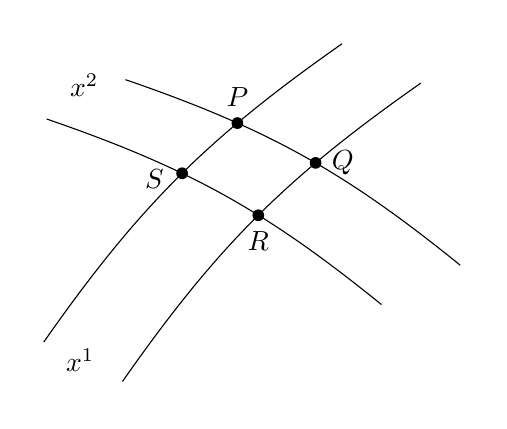
\begin{tikzpicture}
        \node (origin) at (0,0) {}; % Origin node, not shown
        
        %% These are the four corners of the "square"
        \node (a) at (0,0) {};
        \node (b) at (1,-0.5) {};
        \node (c) at (5.5,1) {};
        \node (d) at (4.5,0.5) {};
        \node (e) at (5,3.5) {};
        \node (f) at (4,4) {};
        \node (g) at (1,3.5) {};
        \node (h) at (0,3) {};
        
        %% Curves
        \draw [name path=line-1] (a) to [bend left=10] (f);
        \draw [name path=line-2] (b) to [bend left=10] (e);
        \draw [name path=line-3] (g) to [bend left=10] (c);
        \draw [name path=line-4] (h) to [bend left=10] (d);
        
        %% Points
        \path [name intersections={of=line-1 and line-3,by=P}];
        \node [circle, fill=black,inner sep=1.5pt,label=90:$P$] at (P) {};
        
        \path [name intersections={of=line-2 and line-3,by=Q}];
        \node [circle, fill=black,inner sep=1.5pt,label=0:$Q$] at (Q) {};
        
        \path [name intersections={of=line-2 and line-4,by=R}];
        \node [circle, fill=black,inner sep=1.5pt,label=-90:$R$] at (R) {};
        
        \path [name intersections={of=line-1 and line-4,by=S}];
        \node [circle, fill=black,inner sep=1.5pt,label={[shift={(-0.35,-0.4)}]$S$}] at (S) {};
        
        %% Line labels
        \node [label={[shift={(0.55,-0.5)}]$x^1$}] at (a) {};
        \node [label={[shift={(0.6,0)}]$x^2$}] at (h) {};
    \end{tikzpicture}
    \caption{Labeled diagram of our spacetime $\mathcal{S}$.}
    \label{fig:spacetime_plain}
\end{figure}
\noindent
We can think of the coordinate lines as being like latitude and longitude, or as $(t,x,y,z)$ coordinates.
In the diagram shown above, we're only depicting two coordinate lines, leaving the $x^0$ and $x^3$ coordinates of the points implicit.
Note that in reality, we would be giving names to an infinite number of points, not just the four shown here.
For each of the points shown, there are an associated set of coordinates.
If we take point $Q$ as an example, we might say that $Q$ has coordinates $(x^0,x^1,x^2,x^3)$, or more succinctly that $Q$ has coordinates\footnote{Without rigorously defining it at this point, it's good to recall that we usually think of $x^0$ as being time, while $x^1$ through $x^3$ represent various spatial coordinates. This corresponds nicely with the Minkowsky metric signature.} $x^\mu$.
Note that in this case, this doesn't mean that $x^\mu$ is a member of a vector space, since we haven't talked about what the basis vectors would be; we're just using the superscript notation as a shorthand for each of the separate coordinates.
It's also important to note that we're not talking about any particular coordinate systems here, just a generalized one; it could be spherical or Cartesian or what-not, but for now we really don't care.

Once we've defined a coordinate system, we can start to think of functions on those coordinates.
We could imagine such a function being given by
\[ f(x^\mu) = \mathrm{e}^{x^0}\sin x^1 + \frac{(3x^2)^3}{x^3}. \]
We call any such function a \emph{function on the spacetime}.

\section{Integrating Spacetime and Vector Spaces}
In the past, we've talked about an abstract vector space $V$ with a basis $\{\vec{e}_\mu\}$.
When discussing spacetime, we'll consider a realization of this vector space;
this realized vector space $V$ will be a four-dimensional, real vector space with basis $\{\bm{\partial}_\mu\}$.
Importantly, we won't be creating just one of these vector spaces.
We will create a separate vector space \emph{for each point in spacetime}.
We'll label the vector space by the point it's attached to, so the vector space at $Q$ might be $V_P$.
Because we're creating vector spaces at each point, we also get for free the dual space $V_P^*$ and the infinite number of tensor product spaces associated with $V_P$ and $V^*_P$.

\chapter{Vector and Tensor Fields}
So far, we've created a model of spacetime where each point as an associated set of cordinates $x^\mu$, and is given its own four-dimensional, real vector space $V$ with basis $\{\bm{\partial}_\mu\}$, where $\bm{\partial}_\mu$ is the partial differential operator with respect to the coordinate $x^\mu$.
If we take two points, $P$ and $Q$, and examine arbitrary vectors in their respective vector space, we get vectors $A^\mu \bm{\partial}_\mu \in V_P$ and $B^\mu \bm{\partial}_\mu \in V_Q$.
Although these vector spaces are nearly identical, they aren't the same vector space, so we have to way of comparing the two vectors we've just created.
What distinguishes them are the basis vectors; $\{\bm{\partial}_\mu\}$ represents the differential operators of functions taken at a certain point, so a more complete notation might be $A^\mu \bm{\partial}_\mu \mid_P$ and $B^\mu \bm{\partial}_\mu \mid_Q$.
Because we can no longer be confined to a single vector space, we need a way of talking about what happens in the uncountably infinite number of vector spaces which exist in our spacetime.

\section{Vector Fields}
The solution to this problem is to define what is known as a \emph{vector field}.
Since we've defined a coordinate system $(x^\mu)$ for our spacetime, we can imagine functions of those coordinates such that they are defined for every possible point.
We can then imagine taking the partial derivatives of these functions with respect to each of these coordinates.
\[ \bm{\partial}_\mu f(x^\mu) \tag{defined for every $x^\mu$} \]
We will use these differential operators $\partial_\mu$ as basis vectors in our vector field.
A \emph{vector field} is a collection of vector spaces $V_P$ defined at every point $P$ in a \emph{manifold} (like our spacetime), all of which share a common basis, and some function $f$ defined at those points.
It can be kind of hard to understand the distinction between a vector space and a vector field, so consider this example.
\begin{itemize}
    \item A vector field is like the velocity of wind at every point in a room.
    At each point, we can assign a vector which represents the speed and direction of the wind.
    While these vectors are all broadly measuring the same thing (the velocity of wind), it doesn't really make sense to add these vectors together, since they don't really live in the same space (what does it mean to add the wind at one location to the wind in another?).
    \item A vector space is where each of of those vectors live.
    This is like asking ``at a point $P$, what is every possible direction the wind could be blowing in?''.
    The vector space at point $P$ is separate from the vector space at point $Q$, since the wind at point $P$ isn't necessarily the same as the wind at point $Q$.
\end{itemize}
Mathematically, a vector field is a function
\begin{align*}
    f &: \mathcal{S} \to V_\mathcal{S} \\
      &: P \in \mathcal{S} \mapsto \vec{v} \in V_P
\end{align*}
where $S = \{p\}$ is a subset of our spacetime and $V_\mathcal{S}$ is the vector spaces defined for all point $P$ in $S$.
When we say that $\{\bm{\partial}_\mu\}$ is the basis for the vectors in our vector field, that means that $\bm{\partial}_\mu$ will be the derivative with respect to $x^\mu$ of our vector field (function) $f$ at the point $P$ with coordinates $(x^\mu)$.
In practice, we often leave the function $f$ ambiguous, and treat $\{\bm{\partial}_\mu\}$ as operators for an arbitrary vector field; this is kind of like how we know what the directions in spacetime might be $(t,x,y,z)$ but we don't know exactly \emph{what} we'll be measuring --- maybe it's wind velocity, maybe it's mass flux, maybe it's whatever vector-valued function we want --- but we know we'll be measuring it's rate of change in the directions of $(t,x,y,z)$.
In principle, this means that we can think of an arbitrary vector $A^\mu \bm{\partial}_\mu \in V_P$ in our spacetime as an operator $\mathcal{L}$.
If a function $f$ comes along, $\mathcal{L}$ can operate on it so that we evaluate the partial derivatives of $f$ at a point $P$, so
\[ \mathcal{L}f = A^\mu \bm{\partial}_\mu f \mid_P \;\in \mathbb{R}. \]
This choice of basis $\{\bm{\partial}_\mu\}$ is known as the \emph{coordinate basis}.

\section{Tensors Fields}
We have established that the basis of the vector space $V_P$ at a point $P$ is $\{\bm{\partial}_\mu\}$;
If we want to find the basis of the dual space $V^*_P$ at $P$, we need to find a map which takes a differential operator $\bm{\partial}_\mu$ and gives us a real number.
We call this basis $\{\vec{d}x^\nu\}$, so
\[ \langle \vec{d}x^\nu, \bm{\partial}_\mu \rangle = \delta^\nu_\mu. \]
Elements of $\{\vec{d}x^\nu\}$ are known as \emph{1-forms}. Just as all of the vectors with basis $\{\bm{\partial}_\mu\}$ in $V_\mathcal{S}$ formed a vector field, all of the covectors with basis $\{\vec{d}x^\mu\}$ in $V^*_\mathcal{S}$ form a covector field.
Now that we've defined a basis for the dual space, we can consider tensor product spaces which exist at points in our spacetime.
For example, a $(2,1)$ tensor $T$ would be an element of $V_P \otimes V_P \otimes V^*_P$, and so would have a basis $\bm{\partial}_\lambda \otimes \bm{\partial}_\mu \otimes \vec{d}x^\nu$.
Note that we don't really write which point we're evaluating this basis at; in practice this is contextual, not explicit, and remember that we often won't even write the basis in the first place, and  would just refer to the component $\tensor{T}{^{\lambda\mu}_\nu}$.
One way this is even useful is that we often care about the tensor evaluated at every point in spacetime, not just a particular point, so the ambiguity of the notation can help remind us of that.
Because we're describing tensors at different points in spacetime, we've now created a \emph{tensor field}; just as a vector field assigned vectors to each point in spacetime, a tensor field does the same with tensors.

\section{Vectors and the Coordinate Basis}
As a point of clarification, its helpful to go over exactly what each part of a vector $A^\mu \bm{\partial}_\mu$ in the coordinate basis actually is.
We said that the basis $\{\bm{\partial}_\mu\}$ is differential operators with respect to $x^\mu$ acting on some function $f$, but what about the components?
Well, since $A^\mu$ actually varies with $x^\mu$, we can think of $A^\mu$ as a function on the coordinates $(x^\mu)$.
Explicitly, this would make a vector
\[ A^\nu(x^\mu)\,\bm{\partial}_\nu. \]
Note that here, $(x^\mu)$ represents a point, whereas $\nu$ represents the coordinate directions, so $A^\nu$ contracts with $\partial_\nu$, not with $(x^\mu)$.
We could even replace $(x^\mu)$ with a point $(P)$ to get
\[ A^\nu (P)\, \bm{\partial}_\nu. \]
Because of this, we now have the most explicit form of a tensor yet; for a $(2,2)$ tensor $\Gamma$, we can write it as
\[ \tensor{\Gamma}{^{\alpha\beta}_{\lambda\mu}} = \tensor{\Gamma}{^{\alpha\beta}_{\lambda\mu}} (x^\nu) \,\bm{\partial}_\alpha \otimes \bm{\partial}_\beta \otimes \vec{d}x^\lambda \otimes \vec{d}x^\mu. \]
In practice, we only write out $\tensor{\Gamma}{^{\alpha\beta}_{\lambda\mu}}$, and we have to infer the rest.
Thanks, Index Gymnastics\footnote{If you haven't read any David Sedaris, I \emph{highly} recommend it.}!

\chapter{Coordinate Transformations}
Let's consider our picture of spacetime as we understand in currently.
\begin{figure}[h]
    \centering
    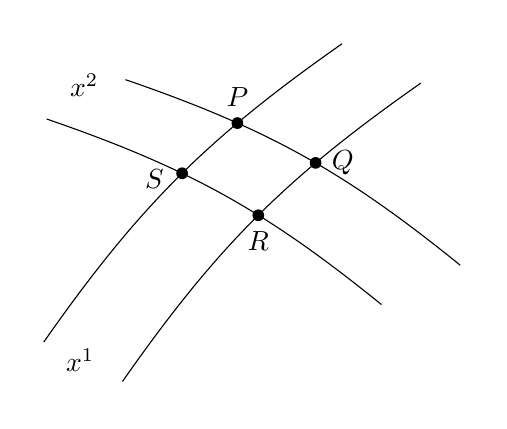
\begin{tikzpicture}
        \node (origin) at (0,0) {}; % Origin node, not shown
        
        %% These are the four corners of the "square"
        \node (a) at (0,0) {};
        \node (b) at (1,-0.5) {};
        \node (c) at (5.5,1) {};
        \node (d) at (4.5,0.5) {};
        \node (e) at (5,3.5) {};
        \node (f) at (4,4) {};
        \node (g) at (1,3.5) {};
        \node (h) at (0,3) {};
        
        %% Curves
        \draw [name path=line-1] (a) to [bend left=10] (f);
        \draw [name path=line-2] (b) to [bend left=10] (e);
        \draw [name path=line-3] (g) to [bend left=10] (c);
        \draw [name path=line-4] (h) to [bend left=10] (d);
        
        %% Points
        \path [name intersections={of=line-1 and line-3,by=P}];
        \node [circle, fill=black,inner sep=1.5pt,label=90:$P$] at (P) {};
        
        \path [name intersections={of=line-2 and line-3,by=Q}];
        \node [circle, fill=black,inner sep=1.5pt,label=0:$Q$] at (Q) {};
        
        \path [name intersections={of=line-2 and line-4,by=R}];
        \node [circle, fill=black,inner sep=1.5pt,label=-90:$R$] at (R) {};
        
        \path [name intersections={of=line-1 and line-4,by=S}];
        \node [circle, fill=black,inner sep=1.5pt,label={[shift={(-0.35,-0.4)}]$S$}] at (S) {};
        
        %% Line labels
        \node [label={[shift={(0.55,-0.5)}]$x^1$}] at (a) {};
        \node [label={[shift={(0.6,0)}]$x^2$}] at (h) {};
    \end{tikzpicture}
\end{figure}
\noindent
Consider the point $Q$.
We can say that $Q$ has coordinates $(q^0, q^1, q^2, q^3) = (q^\mu)$.
Remember that, when dealing with coordinates, the superscript doesn't mean that this transforms like a contravariant vector --- it's just a (canonical) method of indexing the coordinates, and nothing more.
Right now, we are using the $x^\mu$ coordinate system, so each $q^\mu$ is measured with respect to the coordinate lines we've drawn here.
We will introduce a shorthand notation to refer to the coordinates of a point with respect to certain coordinates $x^\mu$:
\[ x^\mu(Q) = x(Q) = (q^0, q^1, q^2, q^3). \]
If it is understood what dimensions we need to represent the coordinates of a point, or we don't care about the distinction, we can simply shorten $x^\mu(Q)$ to $x(Q)$.

\subsection{The Tangent and Cotangent Spaces}
We begin with a really simple renaming; up until now, we've been creating our picture of spacetime and then assigning to each point $P$ a vector space $V_P$ a dual space $V^*_P$.
We defined the basis for $V_P$ to be the collection of differential operators $\{\partial_\mu\}$, and chose a basis $\{\dd{x}^\nu\}$ for $V^*_P$ such that $\langle \dd{x}^\nu, \partial_\mu \rangle = \delta^\nu_\mu$.
We're now going to make the small change of referring to the vector space as the \emph{tangent space} $T_P$, and the dual space as the \emph{cotangent space} $T^*_P$.
We do this because the coordinate basis $\{\partial_\mu\},\{\dd{x}^\nu\}$ is composed of differential operators, which are fundamentally related to the concept of tangency.
Imagine we have some function $\phi(x)$ on our space time and some operator $\mathcal{L} \in T_P$.
If a vector (our operator $\mathcal{L}$) acts on $\phi$ at a point $P$, then we get the directional derivative of $\phi$ at that point.
As a more concrete example, let's say that $\phi(x) = (x^0)^2 + \sin x^3$, and our vector field is $\partial_0 + \partial_3$. Then at a point $Q$, we would see a value
\[ [\partial_0 + \partial_3]\phi(x) = {2x^0 + \cos x^3\mid_Q} = 2q^0 + \cos q^3. \]
Whenever you see a tangent space, remember that it uses the coordinate basis.

It's really important to see that none of this makes any sense until we've established a coordinate system.
Because the coordinate basis gives us directional derivatives \emph{in the direction of the coordinate lines}, if we change our coordinate system our vectors change as well.

\subsection{Arbitrary Change of Bases}
Given a spacetime $\mathcal{S}$, there are an (uncountably) infinite many ways which we can define a coordinate system.
The entire purpose of general relativity is to show the equivalence of these systems, regardless of the basis chosen or the motion of an observer.
As it stands now, our spacetime has at every point a tangent space $T_P$ with basis $\{\partial_\mu\}$, a cotangent space $T^*_P$ with basis $\{\dd{x}^\nu\}$, and the tensor product spaces $\tps{T}^p_q$.
However, as long as we choose a set of linearly independent spanning differential operators from $T_P$, we can create our basis however we like.
Just as with the bases for our regular vector spaces, we can choose a new basis $\partial_{\mu'}$ such that
\[ \partial_{\mu'} = \tensor{\Lambda}{_{\mu'}^\mu}\partial_\mu, \]
where $\tensor{\Lambda}{_{\mu'}^\mu}$ is of course the linear transformation matrix for these two bases.
Technically, since the tangent spaces are independent for each point, we no longer have a single transformation matrix, but rather a transformation which is itself a function on spacetime, so a more complete equation would read
\[ \partial_{\mu'} = \tensor{\Lambda}{_{\mu'}^\mu} (x^\mu)\,\partial_\mu. \]

\subsection{New Coordinate System}
These transformations deal with the case that we want to choose a new basis for our tangent spaces, but we can also consider the case that we change the whole coordinate system itself.
This can be thought of visually as drawing new lines on our spacetime diagram to represent our new coordinate system.
\begin{figure}[h]
    \centering
    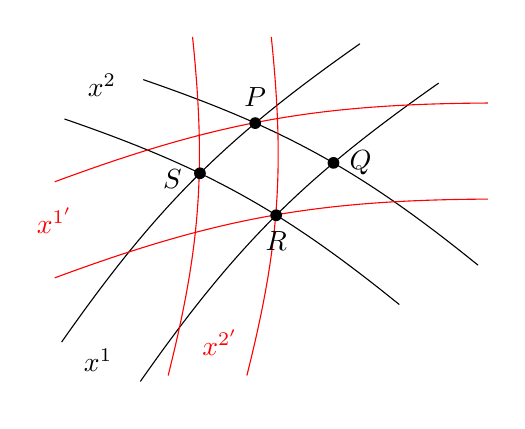
\begin{tikzpicture}
        \node (origin) at (0,0) {}; % Origin node, not shown
        
        %% These are the four corners of the "square"
        \node (a) at (0,0) {};
        \node (b) at (1,-0.5) {};
        \node (c) at (5.5,1) {};
        \node (d) at (4.5,0.5) {};
        \node (e) at (5,3.5) {};
        \node (f) at (4,4) {};
        \node (g) at (1,3.5) {};
        \node (h) at (0,3) {};
        
        %% Curves
        \draw [name path=line-1] (a) to [bend left=10] (f);
        \draw [name path=line-2] (b) to [bend left=10] (e);
        \draw [name path=line-3] (g) to [bend left=10] (c);
        \draw [name path=line-4] (h) to [bend left=10] (d);
        
        %% Alt Curves
        \draw [name path=alt-1, red] (0,2.16) to [bend left=10] (5.5,3.16);
        \draw [name path=alt-2, red] (0,0.94) to [bend left=10] (5.5,1.94);
        \draw [name path=alt-3, red] (1.75,4)  to [bend left=10] (1.44,-0.3);
        \draw [name path=alt-3, red] (2.75,4)  to [bend left=10] (2.44,-0.3);
        
        %% Points
        \path [name intersections={of=line-1 and line-3,by=P}];
        \node [circle, fill=black,inner sep=1.5pt,label=90:$P$] at (P) {};
        
        \path [name intersections={of=line-2 and line-3,by=Q}];
        \node [circle, fill=black,inner sep=1.5pt,label=0:$Q$] at (Q) {};
        
        \path [name intersections={of=line-2 and line-4,by=R}];
        \node [circle, fill=black,inner sep=1.5pt,label=-90:$R$] at (R) {};
        
        \path [name intersections={of=line-1 and line-4,by=S}];
        \node [circle, fill=black,inner sep=1.5pt,label={[shift={(-0.35,-0.4)}]$S$}] at (S) {};
        
        %% Line labels
        \node [label={[shift={(0.55,-0.5)}]$x^1$}] at (a) {};
        \node [label={[shift={(0.6,0)}]$x^2$}] at (h) {};
        
        %% Alt-line Labels
        \node [label={[red]$x^{1'}$}] at (0,1.25) {};
        \node [label={[red]$x^{2'}$}] at (2.1,-0.3) {};
    \end{tikzpicture}
    \caption{Our spacetime $\mathcal{S}$ with coordinate systems $x^\mu$ and $x^{\mu'}$.}
\end{figure}
If we change the coordinates from $(x^\mu)$ to $(x^{\mu'})$, we will necessarily change the coordinate basis as well, since $\{\partial_\mu\}$ is defined with respect to $(x^\mu)$.
Notice, however, that the points themselves don't change, although their coordinates in the respective systems will be different.
The points don't give a damn about which coordinate system is used.

When we talk about changing between coordinate systems, what we really mean are a pair of isomorphisms, $f$ and $f^{-1}$, which act such that
\begin{align*}
    f &: x^\mu \to x^{\mu'}, \\
    f^{-1} &: x^{\mu'} \to x^\mu.
\end{align*}
This means that if we have a point $Q = (q^\mu)$ in the $x^\mu$ system, then $Q$'s coordinates in the $x^{\mu'}$ system will be $f(q^\mu) = (q^{\mu'})$, and that $(q^\mu) = f^{-1} \circ f (q^\mu)$ for all points $Q \in \mathcal{S}$.
As we previously called $x^\mu (Q) = x(x)$ the coordinates in the $x^\mu$ system, we can say that $x^{\mu'}(Q) = x'(Q)$ are the coordinates in the $x^{\mu'}$ system.

Consider that if we have a function $\phi : x^\mu \to \mathbb{R}$ on our spacetime (perhaps representing the strength of an electric field at each point), then we will also need to be able to write some function $\phi' : x^{\mu'} \to \mathbb{R}$ which gives us the same values for the primed coordinates, so that $\phi(Q) = \phi'(Q)$ for all points.
If we want to write $\phi$ as a function of the primed coordinates, we can do so using the coordinate transformations we've just established, so 
\[ \phi(x^\mu) = \phi(f^{-1}(x^{\mu'})) = \phi(x(x^{\mu'})). \]

Even though we've changed the coordinate system of our spacetime, and consequently the basis for our tangent spaces, the tangent spaces themselves really don't change in much the same way that the points in spacetime don't really change.
All we've done is to rename the points, but we haven't changed any of the physics associated with what goes on at those points.
What we have done is change the way that vectors at each point are \emph{written}.
Since $\{\partial_\mu\} \not= \{\partial_{\mu'}\}$, vectors in our tangent space will be written differently depending on which coordinate basis we choose.
We \emph{can}, however, write these new basis vectors as linear combinations of the old basis vectors, which is where the transformation matrix $\tensor{\Lambda}{_{\mu'}^{\mu}}(x)$ comes in.
The the previous section, we were free to choose $\Lambda(x)$ to be whatever we wanted, since we were just defining a new set of basis vectors while the underlying coordinate system remained the same.
Now, however, we've added a constraint.
We need to find the particular $\Lambda$ which is implied by the transformation $f$ between coordinate systems.
If we choose a particular coordinate transformation $f$, we are then \emph{forced} to use a particular basis transformation $\Lambda$ to find $\{\partial_{\mu'}\}$.

\subsection{Finding $\Lambda$ from $f$}
Let's go back to our function $\phi(x(x^{\mu'}))$ on our spacetime.
Since we want the tangent spaces to remain the same under coordinate transformations, we know that we want
\[ \partial_{\mu'} \phi = \partial_\mu \phi \frac{\partial}{\partial{x^{\mu'}}}x(x^{\mu'}), \]
by a simple chain rule expansion.
Since $\phi$ is an arbitrary function, all we really care about is this inner differential, so
\[ \partial_{\mu'} = \partial_\mu \pdv{}{x^{\mu'}}x(x^{\mu'}). \]
This means that 

\[ \Lambda = \pdv{}{x^{\mu'}} x\qty(x^\mu) = \pdv{x^\mu}{x^{\mu'}}, \]
we we simplify $x^\mu = x(x^{\mu'})$.
As a  $4\times 4$ matrix, we would write $\Lambda(x)$ as 
\[ \Lambda = 
    \begin{bmatrix}
        \pdv{x^0}{x^{0'}} & & \\
        & \ddots & \\
        & & \pdv{x^3}{x^{3'}}
    \end{bmatrix}.
\]
\subsection{Transforming the Cotangent Space}
Just as with our ordinary vector space and dual space, we transform the basis of the cotangent space using the inverse transformation as that of the tangent space, so $\dd{x}^{\mu'} = \pdv{x^{\mu'}}{x^\mu} \dd{x}^\mu$, and use the matrix $\Lambda^{-1}(x)$.

\subsection{Requisite Formalism}
When we discussed tensors and vector spaces and tensor product spaces, we did so with a very good degree of formalism.
The lessons started ``from the ground up,'' so to speak, and so they covered everything in depth.
By comparison, the latter parts of the lessons dealing with spacetime and vector fields and such have not really been covered to the same rigor.
Wrapped up in the notion of ``a spacetime $\mathcal{S}$ with a tangent space $T$, a cotangent space $T^*$, and the associated tensor product spaces $\tps{T}^p_q$ affixed to every point'' are the notions of a \emph{manifold}, a \emph{fiber bundle}, and a good deal of topology.
While understanding all of that isn't technically necessary to understanding the following sections, it does help give a good foundation for why all the hand-wavy arguments we've made so far are correct.
If you want to dive into a some (albeit distracting) mathematical formalism for these topics, now would be a good time to pause this lesson and switch to the ``What is a Manifold'' series, and then come back to complete sections 16--39.


\end{document}
